%!TEX root = haiku.tex
\book{\LARGE \FK 日本古典俳句选}

\chapter{\FK 序}

 {\FS

  \hfill\parbox{0.5\textwidth}{\FK
      石蒜香中重把晤,殷殷恰似初逢。百千情事莽盘胸。话澜纷涌处,日影暗移中。余事诗人编简在,词坛更策新功。燕飞掠地雨情浓\footnotemark[1]。相期同奋足,青兕振雄风。

      \hfill——~调寄临江仙
  }

  \footnotetext[1]{\FS 此句本林林某词中的意思。}

  \bigskip

  这是林林重新出来工作相见后,我写给他的一首小词。我不是一个广交游的人。这恐怕跟我的性情和职业都有关系。现在我寓所的小客厅里,每天都不断客人的足迹,有时也因之影响了我作文、读书等工作。但是,说句老实话,真正值得「乐与数晨夕」的「素心人」或像现在普通所说的「老朋友」,实在并不多。在这种仅少的朋友里,林林要算是一个。

  回想起来,我跟林林的交往是久历岁月的。

  最初相识,记得是在海外。当时我们同在东京学习,并且还同在一个学校里,尽管分散在不同部门和年级,也没有在校里碰过头。我们开始接触的情形是相当特殊的。因此,多年以来,它还被保留在我本来不济事的记忆里。时间是三十年代前期的末一、二年(一九三四年或三五年)。一天,我照例从那设在九层楼图书馆的研究室里出来,正走在回寓所去的路上,忽然有人从后面赶来。他走到我的面前时,向我介绍了自己。他就是林林。那时他当然很年轻,躯体修长,面目清秀。见了使我自然地联想起拜伦、雪莱那些诗人穿着翻领衬衣的照片来。应该说,他初次给我的这个印象是令人愉快的。至于我们当时的对话,尽管记不太清楚了,但是,有一点我是没有忘记的,我们谈到亨利·海涅的诗,而且是由他先提起的。他当时正是个「海涅迷」。在海外,此后我们好像没有再晤谈过。那大概因为当时我们彼此都很忙。他正在跟朋友办《质文》一类的杂志,当然还有其它革命工作。我呢,正在利用仅有的时间,研习着图腾主义、太步(禁忌)、巫术等原始文化的问题。

  抗日战争的第二年夏天,我们在当时充满战斗气氛的广州市又碰头了。那时,他在夏衍同志领导的救亡日报社工作,我呢,在四战区政治部。因为共同从事救亡文化活动的关系,我们接触多起来,彼此相互间的了解和关心也增进了。但是,没有多久,敌人在惠州大鹏湾登陆,敌机不断加强对市区的轰炸。广州危在旦夕。我和政治部的同志,是乘这个危城的最后开出的一班火车离开那里的。这时救亡日报社的同志,还在尽最后的努力。

  当我们到了那万头攒动,电灯光显得格外辉煌的火车站,夏衍和林林同志等都赶来送我们。这个不平凡的场面,一直鲜明地深印在我的脑子里。几年后,我在粤北中山大学教书时所做的一首怀念夏衍同志的律诗里,一开头就写述了这个送别的场景
  \begin{center}
      当时感极句难搜,

      危驿千灯照别愁。
  \end{center}

  说是「别愁」,其实是不准确的,至少也是不免简单化了。当时充满我们每位同志的心胸的,是悲愤,火样的悲愤!「别愁」的成分即使存在,也是混和着那种悲愤的。

  林林等离开广州后,徒步往西,最后到了桂林,因为《救亡日报》要在那里继续刊行。后来林林去马尼拉。据说,在它沦陷后,他还在菲律宾境内参加华侨游击队的领导工作,太平洋战争发生后,我们再得不到他的消息,即使是间接的。在坪石——中大临时校址所在地——沦陷前,我写了几首怀人绝句。下面这首,就是关于林林的:
  \begin{center}
      海涅斗心原屹屹,子房风貌乃恂恂。

      南溟劫火横飞后,何处沧波问此人?
  \end{center}

  这首小诗,既提到林林的思想、志向和状貌,又抒写了我怀念的心情。它在我的那个诗组里,恐怕算是写得比较成功的一首吧。林林的爱人很喜欢这首小诗,见面时往往提到它。这也许不仅仅因为他们间的感情关系吧。

  解放战争时期,国民党掌权派感到自己的末日快到了。因此那统治也更加残酷起来。在蒋管区内,不但中共人员受残害或驱逐,连一般民主人士也站不住脚了。我就是在那时被接受了上级「指示」的中大当局强行解聘的。我逃到香港,就在党和民主党派合办的达德学院教书。过了些时候,林林也从马尼拉回来了。我们正好同在一个系(文学系)里,见面谈心的时间就更多了。不能忘记,在芳园(学院的校址)的附近,有一间旧茶馆,是我们学院师生经常在那里吃饭喝茶和谈天的地方,有时学习小组会或工作会,也是在那凉棚底下围着简陋的旧桌子开的。此外,我们还常在当地一些进步的文艺或文化活动的集会上见面。有时,我从学院的青山进市区,晚上回不来了,就在他的寓所里共同打地铺。在这段共同海外流亡的时期里,最值得纪念的,是我曾给他所译的海涅诗集《织工歌》写了序文,那恐怕是到那时为止我所写的第一篇长序了。

  全国解放后,我长住北京,林林开始在广州工作,后来又到印度去办理外事。在那时期里,也偶有把晤的机会,主要是当他到北京述职或开会的时候。而见面机会较多的,还是近几年。不但在参加文艺界的集会时要碰头,偶而,也互相过访。更多的当然是书信的来往。我们就这样渐渐成为老朋友了。在这里,起作用的,除了交往时间长,自然加深了解之外,彼此都喜欢诗歌,在诗学上有互相切磋的要求和活动,这不能不说是一个重要原因吧。

  年来,林林对日本俳句感到很大兴趣。他既和两三同志提倡写「汉俳」(中国式的俳句),又利用工余时间,翻译了近世著名俳谐师松尾芭蕉、与谢芜村和小林一茶三人的作品。他的这种活动,不仅因为对于诗歌的喜爱,也还有想促进国际文化交流的因素在内。最近,他把整理完毕的译诗集的稿子,送给我看,并希望我在前面写一篇序言。他当然知道我不是这方面的专门家,尽管我是颇喜欢这种带有余韵的小诗的。因此,他附带说,要我写序的目的,主要是为了纪念我们的友谊。如果译者要求写的是一篇行家的评论,那么,照道理,我是应该爽直地或婉委地推辞的。但是,译者却是这样的想法,那我又怎么能只顾为自己「藏拙」呢?现在,在序文的开头,我就纵笔写了这么一大篇,说的正是我们交往的经过。自然,序文的内容是不能仅仅以此为满足,它只是一曲前奏罢了。下面我得说说对于俳句的理解和其它一些有关的话头。

  \centerline{\hfill$*$\hfill$*$\hfill}

  俳句是日本传统诗歌形式的一种,是其中形体最小的一种——整首只有十七个音,句调是五、七、五。我们古典诗歌里,词体最短的是「竹枝」,单调的每首二句十四字。其次是「归字谣」,每首十六字。诗体最短的是五言绝句,四句二十个字。但是中国语文,往往一个字(音)就是一个词(当然同时还有一词两字或三字的),它与复音的日本语是不同的。日本的俳句,作为一种独立诗体,成立于十五世纪中,到现在已经四百多年了。据说它是从形体较长的「连歌」的「发句」脱离出来的。自它独立、流行以来,已经产生许多优秀作家(俳谐师)和作品。现在,仍与传统形式的短歌和新体诗等在文坛上乃至于一般社会上流行着,似乎比起我们的旧诗词的形式的传统还更为广泛。在新时代的流传中,它的内容乃至形式不能不有一定程度的改变,这也是很容易理解的事。

  这种形体极小的诗形,到底能不能担任起诗歌(就算抒情诗吧)的任务呢?换一句话,它是否能在一定程度上表达作者的思想、情绪,并且有多少感人的艺术能力呢?这虽然像是一个值得提出的问题,但是,实际已经被它所经历的事实正面回答了。它虽然产生在古代,而且有种种限制,但作为一种传统形式,经过必要的改造,并不是不能生存下去的。事实证明,它是具有相当强韧的生命力的。

  我们试进一步探索这种小形体诗歌的特殊性。它的音数、句数有明显的限制,这是它体裁上的特点。由于这种特点,就产生了一系列的内容选择、表达方式等方面的特殊现象。(自然,从体裁发生史的角度说,它的产生,首先是由于存在着那种要求表现的刹那情思。)具体点说,它所表现的事物和情思,必须是极简单的、压缩的。像叙事诗所表现的那些巨大复杂的故事情节、人物形象以及渗透其中的相应的思想、感情,固然无法受容和表出,就是一般抒情诗(特别是西方式的抒情诗)所表现的事象、景物比较复杂或错综的内容和对它的写法,也是无法办到的。它只能极简洁地含蓄地去表现那些片断的、一闪即逝的景象和情思。它像含苞欲放的花朵,那些花瓣和它的色香,都没有怎样展开和放出。我国古代诗歌史上,曾记载着某些一、两句的诗,如「抱鼓不鸣董少年」、「满城风雨近重阳」,以及「风萧萧兮易水寒,壮士一去兮不复还」,「将军三箭定天山,壮士长歌入汉关」等,大都是大家比较熟悉的。至于那些富有诗趣的、被编入古诗集里的谚语就更多了。现代中国北方民歌中,还有两句成章的信天游(陕北)、爬山歌(内蒙一带)等诗体。我国古今这些小诗,虽然跟日本的俳句乃至川柳,自有它们彼此不同的地方,但是,这种小形体的韵文,在我们文艺(包括民间文艺)领域里并不完全陌生,却是事实。

  由于上面所说的那些特点,俳句在对读者的作用上,主要是暗示的或触发的。读者除对这种特殊诗歌,有一定的理解之外,还必须有相当的生活体验(包括对自然界事物的体验),并善于思索和体味。这样,才能通过它的凝缩的表现去领会作品所含蕴的情思。它像我们对经过焙干的茶叶一样,要用开水给它泡开来。这样,不但可以使它那卷缩的叶子展开,色泽也恢复了(如果是绿茶)。更重要的是它那香味也出来了。对于俳句这种小诗,如果读者不具备上述的那些条件,结果恐怕要像俗话所说的「囫囵吞枣」那样,不知它到底是什么味道了。例如下面这首芭蕉的名作:

  \begin{center}
      古池塘呀,青蛙跳入水声响。\footnotemark[1]
  \end{center}

  \footnotetext[1]{\FS 这里的译文,是从这个集子里引用的。以下同此。}

  这里所表现的,是作者对于那种特殊的闲寂境界的会心。如果我们不知道作者的世界观和世界感(他是一个颇耽闲寂的俳人)及他遇到的那种情景——在极幽寂的境界内忽然听到那种因青蛙跃入而响起的水声,以及这种特殊情景所唤起的作者心理体会(南朝诗人的名句:「蝉噪林逾静,鸟鸣山更幽」,所表现写境界,两者正有相似之处),并细加吟味,那么我们又怎么能深刻地理解它、鉴赏它,并且评价它呢?

  从俳句对内容的表现来看,大致上有两种不同的形态。一种,也许是数量上比较多的一种,只集中地凝缩地表现了作者所经验的景物或事象(包括人物的活动、思想等)。在这里,它并不显露地或比较直接地表示出作者的思想情绪。看来像是纯客观的。但是,细细加以考察,在那被写出的物象或事象的背后(或当中)是潜藏着作者一定的看法和感情的(两者又常常互相胶结着,虽然在这种小诗里,理智的成分往往超过情绪的)。我们试看看下列一些例子:
  \begin{quote}
      春风吹绿三笠山,游人语声喧。

      白雪之下,独活呀,冒出浅紫芽。

      \hfill——~以上芭蕉

      暑天月下人声喧,村民引水入干田。

      风雪夜来人,拔刀喊借宿。

      \hfill ——~以上芜村

      青蛙悠然见青山。

      抓着新熟的瓜,睡着的孩子。

      \hfill ——~以上一茶
  \end{quote}

  这些句子,乍看起来,似乎并不使人感觉得到那些俳谐师们的见解和心情。其实不然,里面正存在着这种心理因素(否则,它还能为诗么?)。例如芭蕉的第二句,他对于那在寒冻里冒出芽来的植物的生命力是深深理解并且给以赞美的。又如一茶的第一句,那悠然看着青山的青蛙的态度和当前境况,不是这位诗人心里所羡慕和神往的么?总之,在俳句里,这种占重要位置的手法,看似限于客观事物的表现,实际是隐藏着主观成分在内的。这和过去所称的我国盛唐诗歌的某种表现法有些接近。所谓「不着一字,尽得风流」,大概正是说的这类境界吧。俳句这种小形体诗,更多地采用这种表现法,是有它一定的理由的。

  但是,在俳句里也有另外一种表现法,那就是在作品里比较显示出作者的心理态度的——有的所呈现的理智或情绪,还是具有相当强度的。例如:
  \begin{quote}
      坟墓也震动,我的哭声似秋风。

      命也如是,只有草笠下,稍得些凉意。

      \hfill ——~以上芭蕉

      踩了亡妻梳子,感到闺房凉意。

      我死葬墓旁,亦愿作枯芒。

      \hfill ——~以上芜村

      我这颗星,在何处寄宿啊,银河?

      瘦青蛙,别输掉,这里有我一茶!

      \hfill ——~以上一茶
  \end{quote}

  这些诗句对内容的表现,显然跟前面那一组的例子很不同。在这些诗句里,作者的思想、感情是跃然纸上,使读者一接触到就会受感染的。芭蕉的第一句,是追悼他的弟子小杉一笑的。在这两句里,不是直接地把这位老师对于早死的门人的满腔感情吐露出来了么?何等强力的诗句!它很像一张拉紧的弓!从这些地方,我们可以明白有人以为这种特殊诗体只能表现比较细微纤弱的感情的看法,是不确当的。主要问题,还在于作者思想、情感的强弱和他的艺术观的倾向。一茶俳句里的思想,用我国古人的话来说是「民胞物与」,用现在的话来说便是「人道主义」或「民主精神」。他这首关于瘦青蛙的俳句,不过是许多同类作品的一首罢了。我们看它在那样仅少的字句里,多么强劲地表达出自己同情弱者的心思!从这个角度说,像芭蕉的「寂静蝉声入岩石」或一茶的「筑摩川蝉声贴在天」等句,都是同一性质的表现法,也都是我上面所说道理的有力证明。

  在这些俳句里,还有一种比较特殊的表现法。那就是句里表现不同感觉的「交错」或「汇通」,即注文里所谓的「通感」。例如「比起石山石,秋风色更白」,「海边暮霭色,野鸭声微白」或「牛棚残暑蚊声暗」(都是芭蕉的句子)。熟悉欧洲近代诗学史的同志大都会知道这种通感法,正是象征主义诗人及同时代其它流派的某些作者所主张或采用过的一种表现法。我国古代诗歌中似乎也偶然出现过这类手法。在俗语里也有时用味觉的「甜」字去形容声音或人的境遇。这种表现法,如果用得恰当,给人的感觉,不但新鲜,而且有时也是深刻的。但是,它的使用领域比较受限制。如果用得不合适(勉强),那就不是诗的辞藻,而是梦呓或疯子的话了。

  文艺作品,是反映人们的社会生活的,是表达作者的思想、想象和情绪的。不管怎样特殊的体裁,对于这种原理是很少例外的。在这个集子的作品里,广泛地反映作者们祖国山川气候、风俗人情、历史人物以及草木鸟兽各方面的情形,自然同时也或明或隐地反映了他们相关联的思想、想象和感情。在这里,特别引起我们注意的,是过去日本人民那些风俗习惯,以及当中不少跟我们国家过去所流行的(有的,现在某些地方还多少有它的余留)民俗活动。这是日本民俗史的重要资料,也是东亚比较民俗学的重要资料。前者,例如盂兰盆节的男女集合舞蹈。男女佣人每年正月和七月十六日放假回家,九月十三夜赏月这些大都是日本民族自己的民俗(有的可能有点大陆风俗的影响)。后者如在正月七日的吃七草粥、五月十三日种竹,认为易生,号「竹醉日」,及小孩生后保存脐带的习俗等,这就跟大陆过去的民间风俗、习惯有极亲密的关系了。孔老夫子对于诗歌的作用,除了兴、观、群、怨之外,并指出「多识鸟兽草木之名」。用我们现在的话来说,就是诗歌除了能给人以精神修养,还能够提供人们所需要的某些实际知识(自然的和社会的知识)。这个俳句集,对于我们的作用也正是这样(尽管需要同时去读译者的注释才能充分得到那些知识)。

  \centerline{\hfill$*$\hfill$*$\hfill}

  中国诗歌,大概千年以前就流传到日本了,并且在那里产生了一定的影响。但是,日本的俳句、短歌,比较认真地介绍入中国,却是在「五四」新文化运动之后(虽然现在算起来,也已经六十多年了)。在那前后被介绍过来的还有法国诗人所仿作的俳句(也可以叫做「法俳」吧?)和印度泰戈尔的小诗(《迷途之鸟》等)。这样就出现了许多爱读者和仿作(后者只是仿作小诗的形式和某些表现手法,并没有,也不可能用原来的格律)。不仅在刊物上多看到这种两三行一首的小诗,而且也有人提出应作这种小诗的主张。根据我的记忆,初期的白话诗人如康白清、俞平伯、徐玉诺、汪静之……都作过这种受日本俳句等影响的小诗,而谢冰心更是写得多和出名的。朱自清的《除夜》,不但我当时反复吟咏过,后来也常常记起它。俞平伯《忆游杂诗》里某些章,情形也有近似之处。我自己呢,记得直到抗日战争后期,还写过这种形式的诗。自然,当时小诗的流行,并不是文艺界所有的人都赞同的。记得有的同志就严厉批评过(所谓「诗之防御战」)。由于新诗的进展和格律诗的提倡等原因,这种小诗活动,后来渐渐退潮了。到了现在,文艺界的同志,不是搞这一段时期的诗歌史的,恐怕连知道的人也很少了(尽管在抗日战争时期,又有人把它跟其它日本诗体的作品介绍过)。

  林林这次不但在新的历史条件下,继续「五四」时期介绍俳句这种小诗的活动,而且在所译作品的数量,及对作者的介绍和作品的注释等方面都做了进一步的工作。尽管因为种种关系,这个译本不能说是完美无缺的,但是,在当前情况下,它的出版,不但需要,而且也是确实有益的。不错,这集子里介绍的是日本近世明治以前的文学作品,时代和作者乃至体裁本身等的限制,是不能免除的。但是,只要我们的读者用鉴别的眼光去观察、学习、品赏这种异国诗歌的历史遗产,我想决不会是徒劳的。我们新诗的创立,尽管已有多年的历史,但是在形式上它还在摸索过程中。现在这种译诗,在某些方面(例如表现的节约、精炼)能给我们一点启示也未可知。

  在这序文将要结束的时候,我想附带说说关于翻译这种小诗所用文字和句调的意见。它或者可供今后继续这方面译业同志的一点参考。「五四」后,译日本俳句和短歌,用的是白话自由体(例如周启明的《日本的诗歌》)。后来有人翻译这类诗歌,基本上却采用文言和旧诗词句调(如钱稻孙的《日本诗歌选》)。现在林林的译文,是两种都用的——对芭蕉、芜村用文言、四句调,对一茶则多用白话和自由体。这两种译法,都有一定的道理,也各有长处。但是我个人粗浅的想法,采用口语和散文体,尽管有它的缺点,如不能保持原诗格律化的的特点,其次,是不大符合中国读者对诗歌的传统审美习惯。但是,它却另有两种颇值得注意的好处:

  (一)它可以尽量保存原文所有的那些表示感情的感叹词,如ヤ、カナ等。在这种小形体抒情诗里,这类感叹词的存在是重要的,它往往有着传神的作用。在另一种译法里,这种词一般就被删去了,它不能不是一种损失。

  (二)如果说文言和传统诗词句调的运用,能照顾到读者的审美习惯,但用白话和自由体,却能产生一种异国情调。它原来是一种外国诗呀!我向来不大喜欢那些用中国五、七言古体诗形式去译西洋近代诗人的作品的作法。这也许是个人的偏见,但我想它也有一定的道理。

  最后,我表示一点虔诚的希望:林林同志或其他有条件和兴趣的同志,能够化功夫译出一些日本从明治以来,直到现在所产生的优秀的俳句或短歌。这种文化作业,同样是我们学界所需要的——我个人也愿作它的一个爱读者呢。

  \hfill 钟敬文

  \hfill 一九八二年十二月十一日北京
 }

\chapter[{\FM 松尾芭蕉}]{\FM \ruby[g]{松}{まつ}\ruby[g]{尾}{お}\ruby[g]{芭}{ば}\ruby[g]{蕉}{しょう}}

\begin{center}
    \begin{figure}
        \centering
        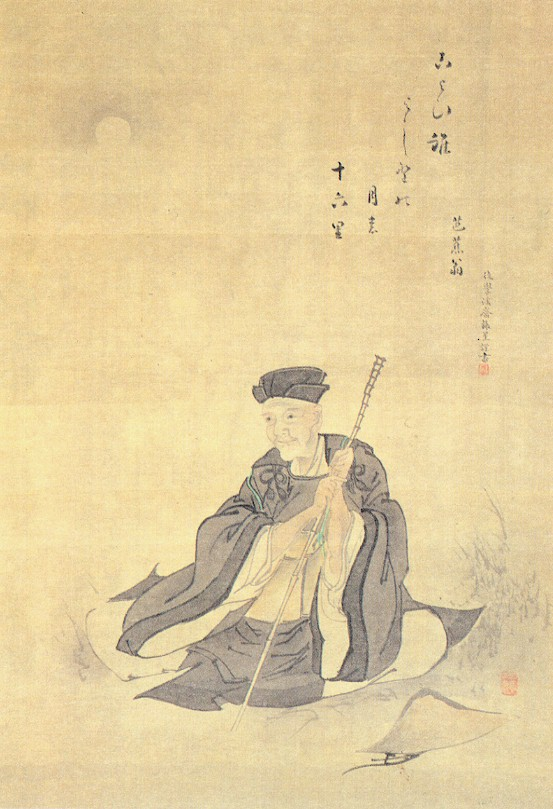
\includegraphics[height=0.9\textheight]{matsuo}\\[1em]
        \large{\FS 松尾芭蕉画像}
    \end{figure}
\end{center}

\newpage

{\FS
    松尾芭蕉(1644—1694)生于伊贺国(今三重县)上野赤坂町下级武士家,原名宗房。幼时陪同藤堂良忠(俳号蝉吟)读书,良忠师事北村季吟,学习贞门俳谐,他对芭蕉有所影响。芭蕉二十三岁时离开家里到京都,向北村季吟学俳谐和古典文学。二十九岁到江户,虽然生活清苦,但努力学俳谐,和当时流行的谈林派俳人交往,也受了影响。三十二岁时,别号桃青,参加西山宗因的俳席。自离开江户城市,过着漂泊的生活,进行艺术的探索,逐渐形成自己的俳风。一六八〇年,三十七岁时,有一批优秀的弟子杉风、卜尺、岚雪、其角等,确立了在俳坛的地位。同年冬,转入隅田川下游东岸的深川六间堀的草庵,以杜甫诗句「门泊东吴万里船」,把草庵称为「泊船堂」,翌年春,在门口种下李下弟子所赠一棵芭蕉,长得茂盛,此庵就叫芭蕉庵,俳号称芭蕉。年底芭蕉庵被别处大火蔓延烧掉,不得不到甲斐国(山梨县)的谷村暂住。一六八三年五月回江户,从此有意过着旅游的生活。一六八四年(四十一岁),开始《野曝纪行》的旅行(又名《甲子行吟》),在名古屋完成第一集《冬日》,奠定了芭蕉风格的基础。翌年四月末回到再建的芭蕉庵,一六八七年八月和弟子曾良、宗波赴常陆国鹿岛旅行写《鹿岛纪行》。十月下旬从江户出发开始《书箱小文》旅行。(《书箱小文》未定稿,后来于一六九一年夏才执笔整理。)归途和弟子越人到信浓国更科,写《更科纪行》。一六八九年三月末带着弟子曾良巡游奥羽北陆,经日光、白河、松岛、平泉、尾花泽、出羽三山、酒田、象潟、出云崎、金泽、福井、敦贺等地,八月下旬至九月初四在大垣停留。全程约二千四百公里,历时六个多月。五年后一六九四年完成《奥州小道》有名的旅行记。他在旅途中,思考诗艺理念问题。一六九〇年,四十七岁,因这次辛苦的旅行,身体不好,移住国分山的幻住庵,出庵前完成《幻住庵记》初稿。一六九一年正月归回故乡伊贺。四五月之间,住在嵯峨落柿舍,留下《嵯峨日记》。九月底离开京都,十月中归回江户,这时已到蕉风的成熟期。芭蕉一生所写的俳谐集有《冬日》、《旷野》、《猿蓑》、《炭包》、《续猿蓑》等七部,这些都是和弟子们一起作的。一六九四年五月又从江户往西旅行,经过奈良,九月末在途中得痢疾,病情恶化,十月八日更深时,给门人支考留下「旅中正卧病,梦绕荒野行」的名句。十月十二日午后在大阪逝世,享年五十一岁。按他的遗嘱,遗体运去葬在膳所的义仲寺内。

    芭蕉经贞门\footnotemark[1]、谈林\footnotemark[2] 两派的俳风,逐步形成自己俳谐的蕉风。到了谈林衰落的后期,他以为作为诗艺的俳谐,当是真诚的,并从传统的继承与发展中,探索新的境界,思考「不易·流行」的艺术观。据研究,所谓「不易」,说的是经越年代还能感人,「流行」说的是随着时代开拓新意境。他认为真诚是俳谐的要素,所谓「不易」与「流行」的作品也是属于同一来源。他要求细致深入地描写对象,钻研美的理念。日本的俳论,一般都称赞他的清寂的代表作「古池塘呀,青蛙跳入响水声」,以一瞬间的小动作的水声,波动了大静的周围,表示作者幽思微情的境界。但是他也写出「坟墓也震动,我的哭声似秋风」那种激情的句子。芭蕉长期旅行接触大自然,写了许多美妙的风光,但也写了一些社会生活,多写自己,也写别人。如「听得猿声悲,秋风又传弃儿啼,谁个最惨凄?」「一年又一年,叫猴戴假面」表现了一定深度的社会性。他常以动物比喻自己,如「离群病雁,落足旅途夜里寒」、「蝴蝶为白罂粟花,撕下翅膀做纪念」等等。

    芭蕉对中国诗文很有素养,他喜爱庄子哲学反俗精神,崇尚杜甫、李白的高逸诗境,这在他的文集句集中反映出来。他把他的处境和心情,写得纯净,富有感人的艺术力。从总体看,他写悲却染有喜色,写喜却含着悲调,晚年要求雅俗浑然融合,创发新意境。他认为平易自然,才是诗艺的妙境。我觉得他晚年许多吟咏秋天情景的作品,饶有这种韵味。

    生活是艺术的源泉,没有旅行,他也就难以写出游记的名作,在游记中闪烁着珠玉般的俳句。他多年漂泊各地,离开城市社会,接触山野人民生活,把深所体会的自然美,升华为艺术美,同时抒写了自己真诚的心灵,创造了独特的艺术风格,也可以说,芭蕉把他的生活沉浸在艺术之中。他的作品,在日本文学史上占有地位,树立了自己的丰碑。他的俳风影响日本俳坛。芭蕉的句碑遍布日本各地,共达三百余座,人们把他尊为「俳圣」。

    \footnotetext[1]{\FS 贞门,松永贞德(1571—1653)拥有一批门徒,倡议不避俗语,但防止过于不雅之词,要求富有生活趣味的诙谐。}

    \footnotetext[2]{\FS 谈林派,以西山宗因(1605—1682)为中心,提倡新风气,倾向市民性,他们的作品的情调较为自由。}
}

\newpage

\section{\FK 新年}

\setcounter{haikucounter}{0}

\begin{haiku}
    {\FH うたがふな、\ruby[g]{潮}{うしお}の花も、浦の春。}

    {\FK 莫疑问,潮头花,亦是滨海春。}
\end{haiku}

\begin{haiku}
    {\FH 元日や、思えばさびし、秋の暮。}

    {\FK 岁旦}

    {\FK 正是年初一,想起暮秋寂寞日。}
\end{haiku}

\begin{haiku}
    {\FH 年々や、猿に着せたる、猿の面。}

    {\FK 一年又一年,叫猴戴假面。}

    {\FT 注:耍猴的,带猴子在肩膀上,挨家逐户打鼓叫猴子跳舞,以求得一点小钱。它和《燕京岁时记》记载的一样,都在新年。此句也有以猴子比喻人的意思。}
\end{haiku}

\begin{haiku}
    {\FH 大津絵の、\ruby[g]{筆}{ふで}のはじめは、何\ruby[g]{仏}{ぼとけ}。}

    {\FK 大津绘,年初落笔是何佛?}

    {\FT 注:大津绘是民间通俗画,元禄年代之前,以佛画居多。岩佐又兵卫擅长佛画,这是作者在人家看到贴着大津绘的即兴句。}
\end{haiku}

\section{\FK 春}

\setcounter{haikucounter}{0}

\begin{haiku}
    {\FH 行く春に、和歌の浦にて、追ひ付きたり。}

    {\FK 和歌浦}

    {\FK 春将归去,追它到和歌浦。}

    {\FT 注:和歌浦在和歌山市南的湾岸一带。}
\end{haiku}

\begin{haiku}
    {\FH 行く春や、鳥啼き魚の、目は泪。}

    {\FK 春将归,鸟啼鱼落泪。}

    {\FT 注:汉诗词常写鱼的自得其乐,宋吴文英《高阳台》却道:「飞红若到西湖底,搅翠澜,总是愁鱼」,适意新颖。芭蕉的鱼落泪,确是不同凡响的佳句。}
\end{haiku}

\begin{haiku}
    {\FH 行く春を、\ruby[g]{近江}{おうみ}の人と、\ruby[g]{惜}{お}しみける。}

    {\FK 望湖水惜春}

    {\FK 我与近江人,同惜春归去。}

    {\FT 注:近江,今滋贺县境内,琵琶湖在这地区。}
\end{haiku}

\begin{haiku}
    {\FH 春なれや、名もなき山の、\ruby[g]{薄}{うす}霞。\footnote{\FT 也有本作《朝霞》。}}

    {\FK 往奈良路上}

    {\FK 春日已来矣,此山何名未得知,薄霭透明媚。}
\end{haiku}

\begin{haiku}
    {\FH 辛崎の、松は花より、\ruby[g]{朧}{おぼろ}にて。}

    {\FK 湖水眺望}

    {\FK 唐崎松比花朦胧。}

    {\FT 注:唐崎,又写作辛崎,在滋贺县大津市琵琶湖的西南岸。在春夜的湖畔,眺望唐崎的松树,为月光映照,浮泛墨绘的景色,看来比那边的樱花更饶朦胧美。}
\end{haiku}

\begin{haiku}
    {\FH 春\ruby[g]{雨}{さめ}や、\ruby[g]{蓬}{よもぎ}をのばす、\ruby[g]{艸}{くさ}の道。}

    {\FK 春雨霏霏芳草径,飞蓬正茂盛。}

    {\FT 注:这句描写春雨,芥川龙之介很赏识它的原句。}
\end{haiku}

\begin{haiku}
    {\FH 春雨や、\ruby[g]{蜂}{はち}の\ruby[g]{巣}{す}つたふ、屋根の\ruby[g]{漏}{も}り。}

    {\FK 屋顶漏春雨,顺着蜂巢点点滴。}

    {\FT 注:屋顶是稻草铺的,芭蕉庵的春雨漏滴声,如在读者心中响着。}
\end{haiku}

\begin{haiku}
    {\FH 水取りや、\ruby[g]{氷}{こおり}の僧の、\ruby[g]{沓}{くつ}の音。}

    {\FK 闲居二月堂}

    {\FK 汲水去,寒僧鞋底声。}

    {\FT 注:奈良东大寺二月堂,二月间有深夜僧众到堂旁若狭井汲水的仪式。僧人穿白衣,举松明,景象十分严肃。}
\end{haiku}

\begin{haiku}
    {\FH 猫の恋、やむとき\ruby[g]{閨}{ねや}の、朧月。}

    {\FK 猫儿叫春停歇时,闺中望见朦胧月。}

    {\FT 注:「猫恋」是俳谐最初季语化的素材。贞门、谈林两派较多吟咏。}
\end{haiku}

\begin{haiku}
    {\FH 鶯や、柳のうしろ、\ruby[g]{薮}{やぶ}の前。}

    {\FK 黄鹂声声啭,听来刚在翠柳后,又在竹林前。}
\end{haiku}

\begin{haiku}
    {\FH 原中や、ものにもつかず、啼く\ruby[g]{雲雀}{ひばり}。}

    {\FK 云雀原野鸣,自由自在一心轻。}
\end{haiku}

\begin{haiku}
    {\FH 雲雀より、空にやすらふ、\ruby[g]{峠}{とうげ}かな。}

    {\FK 脐峠}

    {\FK 小憩于参天峰顶,云雀在下飞鸣。}

    {\FT 注:脐峠今为细峠(奈良县吉野郡吉野町)位于樱井到吉野途中。峠是山巅之意。}
\end{haiku}

\begin{haiku}
    {\FH \ruby[g]{盃}{さかずき}に、\ruby[g]{泥}{どろ}な\ruby[g]{落}{おと}しそ、\ruby[g]{群}{むら}燕。}

    {\FK 楠边}

    {\FK 群燕低飞,碎泥落酒杯。}

    {\FT 注:楠边为朝熊山西麓村落。}
\end{haiku}

\begin{haiku}
    {\FH 古池や、\ruby[g]{蛙}{かわず}飛びこむ、水の音}

    {\FK 古池塘呀,青蛙跳入水声响}

    {\FT 注:这是芭蕉的名作,表示深得清寂幽玄的意境。}
\end{haiku}

\begin{haiku}
    {\FH 蝶よ蝶よ、\ruby[g]{唐土}{もろこし}の、俳諧\ruby[g]{問}{と}はん。}

    {\FK 拜庄周尊像}

    {\FK 蝴蝶哟,蝴蝶,请问何为唐土俳谐。}

    {\FT 注:取庄周梦蝴蝶典故,俳谐含有寓言的意思。}
\end{haiku}

\begin{haiku}
    {\FH 君や蝶、我や\ruby[g]{荘子}{さうじ}が、夢心。}

    {\FK 你哟蝴蝶,我哟庄子,梦之心。}

    {\FT 注:据一六九〇年四月十日书简,芭蕉与怒谁谈论自然之道,十分默契,写此赠句。怒谁和芭蕉都是《庄子》的热心读者。}
\end{haiku}

\begin{haiku}
    {\FH 物好きや、匂はぬ草に、とまる蝶。}

    {\FK 无香杂草里,好奇蝴蝶不离去。}

    {\FT 注:这是作者背离世俗的自喻句。}
\end{haiku}

\begin{haiku}
    {\FH 梅白し、昨日や鶴を、\ruby[g]{盗}{ぬす}まれし。}

    {\FK 梅林}

    {\FK 白梅开正好,白鹤昨天可被盗?}

    {\FT 注:梅林乃京都富豪谈林派俳人三井秋风的别墅。梅鹤风雅,出自林和靖的典故。只见梅不见鹤,以为是被盗了,真煞风景。}
\end{haiku}

\begin{haiku}
    {\FH 忘るなよ、薮の中なる、梅の花。}

    {\FK 莫忘记,梅开在草丛里。}

    {\FT 注:这是赠别句,在草丛里的梅花,喻芭蕉自己。}
\end{haiku}

\begin{haiku}
    {\FH 里の子よ、梅折り残せ、牛の\ruby[g]{鞭}{むち}。}

    {\FK 梅枝作牛鞭,村童哟,请莫折尽。}

    {\FT 注:写村野的情趣。唐朝李群玉咏梅句有「已被儿童苦攀折,更遭风雨损馨香」的诗句。}
\end{haiku}

\begin{haiku}
    {\FH 水鳥の、はしに付たる梅白し。}

    {\FK 水鸟嘴,沾有梅瓣白。}

    {\FT 注:郭沫若以为此作比白居易《春至》诗句「白片落梅浮涧水」更形象化。}
\end{haiku}

\begin{haiku}
    {\FH \ruby[g]{暖簾}{のうれん}の、奥ものふかし、北の梅。}

    {\FK 一有之妻}

    {\FK 暖帘之内,可爱北堂梅。}

    {\FT 注:北堂梅花指一有之妻女俳人斯波园女。园女乃伊势山田秦师贞之女,嫁与同地医师斯波一有为妻,是蕉风门人。}
\end{haiku}

\begin{haiku}
    {\FH 人も見ぬ、春や鏡の、裏の梅。}

    {\FK 无人探春来,镜里梅自开。}

    {\FT 注:镜是古时铜镜。背面铸有梅花,用返照的句法,芭蕉以此自喻。}
\end{haiku}

\begin{haiku}
    {\FH \ruby[g]{数}{かぞ}へ来ぬ、屋敷屋敷の、梅柳。}

    {\FK 缓步}

    {\FK 一路数着来,府邸、府邸之梅柳。}
\end{haiku}

\begin{haiku}
    {\FH 梅が\ruby[g]{香}{か}に、のつと日の出る、山\ruby[g]{路}{じ}哉。}

    {\FK 梅花山路飘香,朝阳猛然出现。}
\end{haiku}

\begin{haiku}
    {\FH 雪\ruby[g]{間}{ま}より、薄紫の、芽\ruby[g]{独活}{うど}哉。}

    {\FK 白雪下,独活呀,冒出浅紫芽。}

    {\FT 注:独活即土当归。此句写白紫对照,新生命的出现。}
\end{haiku}

\begin{haiku}
    {\FH 咲き\ruby[g]{乱}{みだ}す、桃の中より、初櫻。}

    {\FK 桃花丛中见早樱。}
\end{haiku}

\begin{haiku}
    {\FH うち山や、\ruby[g]{外様}{とざま}しらずの、花\ruby[g]{盛}{ざか}り。}

    {\FK 内山花多娇,外人哪知晓。}
\end{haiku}

\begin{haiku}
    {\FH \ruby[g]{鸛}{こふ}の巣に、嵐の\ruby[g]{外}{ほか}の、櫻哉。}

    {\FK 山家}

    {\FK 鹳巢高,山风外樱花闹。}

    {\FT 注:鹳形似鹤,巢筑在高树上。似拟山家主人的口气,讲环境的优越。}
\end{haiku}

\begin{haiku}
    {\FH 木のもとに、\ruby[g]{汁}{しる}も\ruby[g]{膾}{なます}も、桜かな。}

    {\FK 赏花}

    {\FK 树下鱼肉丝、菜汤上,飘落樱花瓣。}

    {\FT 注:记与伊贺人们一起赏樱。历来写樱花很多,这里有鱼肉丝、菜汤的生活气息,显示出平民性。}
\end{haiku}

\begin{haiku}
    {\FH \ruby[g]{阿}{お}蘭\ruby[g]{陀}{だ}も、花に来にけり、馬に\ruby[g]{鞍}{くら}。}

    {\FK 荷兰人,马挂鞍来赏樱。}

    {\FT 注:荷兰驻长崎商馆馆长,每年到江户赏樱,并拜谒江户将军。}
\end{haiku}

\begin{haiku}
    {\FH 京は九万、九千くんじゅの、花見哉。}

    {\FK 京都看花天,群集九万九千。}
\end{haiku}

\begin{haiku}
    {\FH 花にうき世、我が酒白く、飯黒し。}

    {\FK 忧方知酒圣,贫始觉钱神}

    {\FK 对花忧人间,我酒浊饭淡。}

    {\FT 注:题是白居易《江南谪居十韵》的诗句。}
\end{haiku}

\begin{haiku}
    {\FH 花咲きて、七日鶴見る、\ruby[g]{麓}{ふもと}哉。}

    {\FK 三月廿日即兴}

    {\FK 山麓花盛开,七天鹤常在。}

    {\FT 注:比睿山麓,花开春色美好,白鹤在那周内也飞来玩赏。}
\end{haiku}

\begin{haiku}
    {\FH 花の雲、\ruby[g]{鐘}{かね}は上野か、浅草か。}

    {\FK 草庵}

    {\FK 花云缥缈,钟声来自上野,还是浅草?}

    {\FT 注:花云指樱花如轻云。该庵在江户郊外,可以听到上野或浅草的钟声。}
\end{haiku}

\begin{haiku}
    {\FH 何の木の、花とはしらず、匂かな。}

    {\FK 伊势山田}

    {\FK 不知何树花开,香气扑鼻来。}
\end{haiku}

\begin{haiku}
    {\FH しばらくは、花の上なる、月夜かな。}

    {\FK 春月夜,暂且逗留花蕊上。}

    {\FT 注:花即樱花,这是描绘月和花的静美。}
\end{haiku}

\begin{haiku}
    {\FH 四方より、花吹き入れて、鳰の波。}

    {\FK 洒落堂记}

    {\FK 四方飘下花雪来,尽归䴙䴘海。}

    {\FT 注:四方即琵琶湖四周,指唐崎、比睿、比良、三上诸山。䴙䴘是一种水鸟,俗称水葫芦,琵琶湖又称䴙䴘海。这是写从洒落堂(主人是滨田珍夕医师)眺望琵琶湖的春日风光。}
\end{haiku}

\begin{haiku}
    {\FH 年々や、桜を\ruby[g]{肥}{こ}やす、花の\ruby[g]{塵}{ちり}。}

    {\FK 年年樱瓣飞,花屑化作肥。}

    {\FT 注:这是落红化作春泥的意思。}
\end{haiku}

\begin{haiku}
    {\FH わが\ruby[g]{衣}{きぬ}に、\ruby[g]{伏見}{ふし}の桃の、雫せよ。}

    {\FK 伏见西岸寺遇任口上人}

    {\FK 请将伏见桃花露,滴落我衣襟。}

    {\FT 注:伏见为京都市南区一部,一五九四年丰臣秀吉在桃山筑伏见城,该城为桃名所。任口上人在西岸寺任职,芭蕉尊重这位老前辈。}
\end{haiku}

\begin{haiku}
    {\FH \ruby[g]{草臥}{くたぶ}れて、\ruby[g]{宿}{やど}かる頃や、藤の花。}

    {\FK 太和行脚时}

    {\FK 投宿已疲乏,忽又见藤花。}

    {\FT 注:藤花在暮霭中有凋谢状,看了更感困倦。}
\end{haiku}

\begin{haiku}
    {\FH ほろほろと、山吹ちるか、滝の音。}

    {\FK 西河}

    {\FK 棣棠落花簌簌,可是激湍漉漉?}

    {\FT 注:写和歌山县吉野川岸畔的景致。原文有双声的句法。}
\end{haiku}

\begin{haiku}
    {\FH 菜\ruby[g]{畠}{ばたけ}に、花見顔なる、\ruby[g]{雀}{すずめ}哉。}

    {\FK 行吟}

    {\FK 菜花开满园,麻雀赏花颜。}
\end{haiku}

\begin{haiku}
    {\FH \ruby[g]{躑躅}{つつじ}生けて、その陰に\ruby[g]{干鱈}{ひだら}、\ruby[g]{割}{さ}く女。}

    {\FK 坐在茶店午休}

    {\FK 桶内插杜鹃,阴凉里,女佣撕裂鳕鱼干。}

    {\FT 注:写客栈女佣撕鳕鱼,准备客饭,可看出俳谐的生活化、通俗化。}
\end{haiku}

\begin{haiku}
    {\FH 山路来て、何やらゆかし、菫草。}

    {\FK 越过山道,去大津路上}

    {\FK 山路费攀登,竟有可爱紫地丁。}
\end{haiku}

\begin{haiku}
    {\FH よく見れば、\ruby[g]{薺}{なずな}花咲く、\ruby[g]{垣}{かき}根かな。}

    {\FK 细看墙根下,竟然开荠花。}

    {\FT 注:白居易诗句有「惆怅去年墙下地,今春唯有荠花开」。情景相似。}
\end{haiku}

\begin{haiku}
    {\FH \ruby[g]{衰}{おとろ}ひや、歯に喰ひ\ruby[g]{当}{あ}てし、\ruby[g]{海苔}{のり}の砂。}

    {\FK 啮到紫菜砂,感叹老衰牙。}
\end{haiku}

\section{\FK 夏}

\setcounter{haikucounter}{0}

\begin{haiku}
    {\FH 六月や、峰に雲置く、嵐山。}

    {\FK 嵯峨}

    {\FK 六月岚山云遮峰。}

    {\FT 注:六月炎暑,岚山满山苍翠,夏云遮掩山峰。岚山在京都市西部嵯峨地区,在大堰川右岸,自平安朝以来,为红叶与樱花的名所。}
\end{haiku}

\begin{haiku}
    {\FH 秋近き、心の寄るや、四\ruby[g]{畳}{じょう}半。}

    {\FK 元禄七年六月廿一日于大津木节家}

    {\FK 秋近心相连,四席半。}

    {\FT 注:元禄七年一六九四年,芭蕉与各务支考、广濑惟然聚会于望月木节家,在四席半小房间,设有俳谐席。}
\end{haiku}

\begin{haiku}
    {\FH 五月雨に、鳰の浮巣を、見にゆかん。}

    {\FK 致露沾公}

    {\FK 黄梅雨里,看䴙䴘浮巢去}

    {\FT 注:露沾公乃磐城内藤义英,江户俳坛的后援人。}
\end{haiku}

\begin{haiku}
    {\FH 五月雨に、隠れぬものや、瀬田の橋。}

    {\FK 湖景遮掩梅雨中,濑田桥横。}

    {\FT 注:这像一幅浮世绘名家广重的画。濑田桥为日本三大桥之一。}
\end{haiku}

\begin{haiku}
    {\FH 五月雨の、降り残してや、\ruby[g]{光堂}{ひかりどう}。}

    {\FK 梅雨落剩一光堂。}

    {\FT 注:光堂即金色堂。一一八五年为藤原洁衡所建,作为自己死后的坟墓。据记载佛殿内外,施贴金箔,镂嵌螺钿,极尽庄严豪华之美。此句指几百年来年年落梅雨,于今光堂仍辉煌地存在着。}
\end{haiku}

\begin{haiku}
    {\FH 降る音や、耳も\ruby[g]{酸}{す}うなる、梅の雨。}

    {\FK 梅雨声不断,耳朵也发酸。}

    {\FT 注:酸和梅是相关语。这是芭蕉二十三岁时的吟句。}
\end{haiku}

\begin{haiku}
    {\FH 五月雨を、集めて早し、最上川。}

    {\FK 梅雨收集遍,奔流最上川。}

    {\FT 注:最上川在山形县境内,为日本三大急流之一。}
\end{haiku}

\begin{haiku}
    {\FH 松杉を、ほめてや風の、かをる音。}

    {\FK 在小仓山常寂寺}

    {\FK 赞美松杉,薰风声喧。}

    {\FT 注:小仓山在嵯峨里面,松杉翠绿,薰风南来,好似赞美它们一样。}
\end{haiku}

\begin{haiku}
    {\FH このあたり、目に見ゆるものは、皆涼し。}

    {\FK 十八楼记}

    {\FK 望此方,眼底景物皆清凉。}

    {\FT 注:十八楼乃稻叶山麓加岛鸥步(歧阜俳人)的水楼,可以眺望长良川远近的农村渔村和北部的群山诸景。}
\end{haiku}

\begin{haiku}
    {\FH 涼しさを、絵にうつしけり、\ruby[g]{嵯峨}{さが}の竹。}

    {\FK 野明家}

    {\FK 嵯峨竹,清凉入画图。}

    {\FT 注:野明即奥西善六,居嵯峨,称坂井作大夫。嵯峨在京都市西部,多竹。}
\end{haiku}

\begin{haiku}
    {\FH \ruby[g]{蛸壺}{たこつぼ}や、はかなき夢を、夏の月。}

    {\FK 明石夜泊}

    {\FK 夏月夜,章鱼壶中虚幻梦。}

    {\FT 注:明石在兵库县南部,面临播磨滩,那里有陶壶捕章鱼的办法。这是写章鱼已经被捕了,还在做梦。}
\end{haiku}

\begin{haiku}
    {\FH さざれ蟹、足\ruby[g]{這}{は}ひのぼる、清水哉。}

    {\FK 螃蟹小又细,爬上我双足,泉水多清冽。}
\end{haiku}

\begin{haiku}
    {\FH 馬ぼくぼく、我を絵に見る、夏野かな。}

    {\FK 画赞}

    {\FK 马蹄迟迟夏野行,看我身在画图中。}
\end{haiku}

\begin{haiku}
    {\FH \ruby[g]{笈}{おい}も\ruby[g]{太刀}{たち}も、\ruby[g]{五月}{さつき}に飾れ、紙\ruby[g]{幟}{のぼり}。}

    {\FK 大刀与背箱,可同纸旗装饰五月天。}

    {\FT 注:源义经的大刀、弁庆的背箱。源义经(1159—1189)镰仓初期名将,源义朝第九子,扶助其兄源赖朝,讨伐源义仲,又在坛浦击灭平氏。为其兄赖朝所忌,终于被迫自杀。弁庆(?—1189)僧人,义经的从臣,为义经而战死。纸旗画鲤鱼或钟馗等,在端午节前后挂在空中。}
\end{haiku}

\begin{haiku}
    {\FH おもしろうて、やがて悲しき、\ruby[g]{鵜舟}{うぶね}かな。}

    {\FK 鸬鹚船,兴致舒畅,黯然转神伤。}

    {\FT 注:芭蕉在歧阜长良川即景句。捕取鲇鱼的鸬鹚船,先是点燃熊熊的篝火,顺流而下,篝火渐渐消灭,船在黑暗中归去。作者以「欢乐尽而情深」的心理写出。}
\end{haiku}

\begin{haiku}
    {\FH 涼ぬとて、切りぬけにたり、北の窓。}

    {\FK 请纳凉,北墙凿通个小窗。}

    {\FT 注:郭沫若以为此作与汉诗「暑月贫家何所有,客来惟赠北窗风」相近。}
\end{haiku}

\begin{haiku}
    {\FH 雲の峰、いくつ崩れて、月の山。}

    {\FK 几道云峰解散,新月耀辉东土。}

    {\FT 注:《奥州小道》记月山、羽黑山和汤殿山为出羽三山的高峰,句将月山拆开描写。}
\end{haiku}

\begin{haiku}
    {\FH 命なり、わづかの笠の、下涼み。}

    {\FK 佐夜中山}

    {\FK 命也如是,只有草笠下,稍得些凉意。}

    {\FT 注:佐夜中山,今静冈县小笠、榛原二郡之间险峻的山道。当越此山时,一路不见树荫,炎热焦灼,故发此感慨。}
\end{haiku}

\begin{haiku}
    {\FH 降らずとも、竹\ruby[g]{植}{う}うる日は、\ruby[g]{蓑}{みの}と笠。}

    {\FK 竹}

    {\FK 种竹日,不下雨,也要蓑和笠。}

    {\FT 注:种竹日来自中国「竹醉日」即五月十三日,该日种竹易活。因是梅雨时节,故要蓑和笠。}
\end{haiku}

\begin{haiku}
    {\FH \ruby[g]{鹿}{しか}の\ruby[g]{角}{つの}、まづ\ruby[g]{一節}{ひとふし}の、わかれかな。}

    {\FK 奈良别旧友}

    {\FK 鹿角首节先分枝。}

    {\FT 注:旧友指从伊贺故乡来的猿虽、卓袋诸人。最初的鹿角分枝,表示不得不离的意思。这是酬唱之作。}
\end{haiku}

\begin{haiku}
    {\FH ほととぎす、消え行く方や、島一つ。}

    {\FK 杜鹃飞去已无声,那方只余孤岛景。}

    {\FT 注:据纪行《书箱小文》,从铁拐山向海上瞭望的岛,即淡路岛。该岛在神户西部须磨海岸附近。}
\end{haiku}

\begin{haiku}
    {\FH \ruby[g]{一声}{ひとこえ}の、江に横\ruby[g]{たふ}{とう}や、ほととぎす。}

    {\FK 时鸟声横江水上。}

    {\FT 注:「横江」据说来自《前赤壁赋》的「白露横江,水光接天」和《后赤壁赋》的「适有孤鹤,横江东来」。}
\end{haiku}

\begin{haiku}
    {\FH 鶯や、竹の子薮に、\ruby[g]{老}{おい}を鳴く。}

    {\FK 笋竹丛中莺声老。}

    {\FT 注:芭蕉自老莺,看新生笋竹,便感叹起老来。}
\end{haiku}

\begin{haiku}
    {\FH \ruby[g]{閑}{しずけ}さや、\ruby[g]{岩}{いわ}にしみ入る、蝉の声。}

    {\FK 静寂呀,蝉声入岩石。}

    {\FT 注:此句可与王籍诗「蝉噪林愈静,鸟鸣山更幽」比,作此是因蝉噪、鸟鸣才显得环境更幽静。}
\end{haiku}

\begin{haiku}
    {\FH やがて死ぬ、けしきは見えず、蝉の声。}

    {\FK 无常迅速}

    {\FK 知了在叫,不知死期快到。}

    {\FT 注:有庄子《逍遥游》「蝼蛄不知春秋」句意}
\end{haiku}

\begin{haiku}
    {\FH 草の葉を、落つるより飛ぶ、蛍哉。}

    {\FK 萤火虫,刚落下草丛,就从草丛飞升。}

    {\FT 注:这是抓住两个动作的瞬间,微妙地表示萤火虫的形态。}
\end{haiku}

\begin{haiku}
    {\FH \ruby[g]{蚤虱}{のみしらみ}、馬の\ruby[g]{尿}{ばり}する、枕もと。}

    {\FK 蚤虱横行,枕畔又闻马尿声。}

    {\FT 注:《奥州小道》的旅行,记在尿前山区中寄宿农家,人马同室的情景。}
\end{haiku}

\begin{haiku}
    {\FH 若\ruby[g]{葉}{ば}して、\ruby[g]{御目}{おんめ}の雫、ぬぐはばや。}

    {\FK 新叶滴翠,摘来拂拭尊师泪。}

    {\FT 注:这是到奈良唐招提寺,拜谒盲圣鉴真像之句。}
\end{haiku}

\begin{haiku}
    {\FH あらたふと、青葉若葉の、日の光。}

    {\FK 访日光山}

    {\FK 好辉煌,浓淡绿叶映日光。}

    {\FT 注:一六八九年四月一日,参谒日光东照宫时所作。}
\end{haiku}

\begin{haiku}
    {\FH 須磨\ruby[g]{寺}{でら}や、吹かぬ\ruby[g]{笛}{ふえ}聞く、\ruby[g]{木}{こ}下闇。}

    {\FK 须磨寺,树荫暗处,听此不吹笛。}

    {\FT 注:须磨寺在神户市须磨区,即上野山福祥寺。该寺有名贵文物——平敦盛的青叶笛。源平在一谷会战时,平敦盛腰间挂着心爱的笛子。这是芭蕉的幻想句,想象听到昔日的笛声。}
\end{haiku}

\begin{haiku}
    {\FH \ruby[g]{駿}{する}\ruby[g]{河}{が}路や、花橘も、茶の匂ひ。}

    {\FK 入骏河国}

    {\FK 骏河路上,花桔发茶香。}

    {\FT 注:骏河路,在静冈地区,这条路上,到处白橘花盛开。这里又是制茶的地方,橘花香中也有茶香。}
\end{haiku}

\begin{haiku}
    {\FH \ruby[g]{杜若}{かきつばた}、\ruby[g]{語}{かた}るも旅の、ひとつかな。}

    {\FK 在大阪}

    {\FK 杜若作话题,也是一种旅中趣。}

    {\FT 注:杜若,生在水边,初夏开紫花,又名燕子花。这是旅中与门徒小杉一笑交谈的即兴句。}
\end{haiku}

\begin{haiku}
    {\FH \ruby[g]{菖蒲}{あやめ}草、足に\ruby[g]{結}{むすば}ん、\ruby[g]{草履}{わらじ}の緒。}

    {\FK 菖蒲结做草鞋带,绑在行脚上。}

    {\FT 注:端午节挂菖蒲在檐下避邪,现在绑在脚上,为旅行吉利。}
\end{haiku}

\begin{haiku}
    {\FH 白\ruby[g]{芥子}{げし}に、羽もぐ蝶の、形見かな。}

    {\FK 蝴蝶为白罂粟花,撕下翅膀作纪念。}

    {\FT 注:写他与弟子杜国惜别的强烈感情。蝴蝶比自己,白罂粟比杜国。}
\end{haiku}

\begin{haiku}
    {\FH 撫子に、かかる涙や、\ruby[g]{楠}{くす}の露。}

    {\FK 正成之像\\铁肝石心此人之情}

    {\FK 楠露滴落石竹泪。}

    {\FT 注:写楠木正成(1294—1336)父子在樱井驿诀别悲剧(《太平记》卷一六)的画赞,把石竹当作当时十一岁的正行,把楠木叶滴落的露,作力父亲慈爱的泪,泪滴在树荫下开花的石竹上。}
\end{haiku}

\begin{haiku}
    {\FH 世の人の、見付けぬ花や、\ruby[g]{軒}{のき}の\ruby[g]{栗}{くり}。}

    {\FK 不为世人注意,檐下栗花枝。}
\end{haiku}

\begin{haiku}
    {\FH \ruby[g]{象潟}{きさがた}や、雨に\ruby[g]{西施}{せいし}が、\ruby[g]{合歓}{ねぶ}の花。}

    {\FK 象潟合欢,恰似雨中西施。}

    {\FT 注:象潟今秋田县由利郡象潟汀海滨,雨中合欢花像颦眉泪湿的西施。}
\end{haiku}

\begin{haiku}
    {\FH 朝露や、よごれて涼し、\ruby[g]{瓜}{うり}の泥。}

    {\FK 在去来别墅}

    {\FK 朝露湿瓜泥,黑汙而冷冽。}

    {\FT 注:向井去来乃蕉门十哲之一。芭蕉在夏天早晨步入瓜田地,看到露水和泥土的即景句。}
\end{haiku}

\begin{haiku}
    {\FH 夏来ても、ただひとつ葉の、一葉かな。}

    {\FK 虽是夏天来,石苇依然只一叶。}

    {\FT 注:石苇是生于山野的羊齿类,只长强韧的一片长叶,寒冬不枯萎。这含有孤高之意。}
\end{haiku}

\begin{haiku}
    {\FH 清滝や、波に散り込む、青松葉。}

    {\FK 清泷眺望}

    {\FK 松叶青青,散落清泷波心。\footnote{\FT 此为芭蕉去世前三日在大阪所做。}}

    {\FT 注:清泷即清泷川,在京都郊外梅尾高山寺前流入大堰川,流狭水清。落在波心的,是被薰风刮下的青松叶,并非落叶。}
\end{haiku}

\begin{haiku}
    {\FH 夏草や、\ruby[g]{兵}{つわもの}どもが、夢の跡。}

    {\FK 在奥州高馆}

    {\FK 长夏草木深,武士当年梦痕。}

    {\FT 注:高馆是为源义经建筑的城楼。武士指为源义经而战的家臣。}
\end{haiku}

\begin{haiku}
    {\FH 夏草に、富貴を飾れ、蛇の\ruby[g]{衣}{きぬ}。}

    {\FK 繁茂夏草里,装点富贵蛇衣。}

    {\FT 注:这是在幻住庵的吟作。蛇衣外观华丽,故云能装点富贵。}
\end{haiku}

\section{\FK 秋}

\setcounter{haikucounter}{0}

\begin{haiku}
    {\FH 初秋や、海も青田も、一みどり。}

    {\FK 鸣海眺望}

    {\FK 初秋时节,碧海青田一色。}

    {\FT 注:鸣海,今名古屋市绿巴鸣海町,附近海岸称为鸣海湾。}
\end{haiku}

\begin{haiku}
    {\FH 牛部屋に、\ruby[g]{蚊}{か}の声暗き、残暑哉。}

    {\FK 牛棚残暑蚊声暗。}

    {\FT 注:牛棚暗,听蚊声也暗。这与「鸭声白」同是「通感」句法。初稿是「秋声起,牛棚蚊声低。」}
\end{haiku}

\begin{haiku}
    {\FH 野ざらしを、心に風の、しむ身かな。}

    {\FK 此身或将曝荒原,风吹入骨寒。}

    {\FT 注:一六八四年秋,从江户出发长途旅行,此是《野曝纪行》的首句。}
\end{haiku}

\begin{haiku}
    {\FH 枯枝に、\ruby[g]{烏}{からす}のとまりたるや、秋の暮。}

    {\FK 寒鸦宿枯枝,深秋日暮时。}

    {\FT 注:拟汉诗句题材,有古典情趣。使人忆起马致远《天净沙》「枯藤老树昏鸦」句。}
\end{haiku}

\begin{haiku}
    {\FH この道を、行く人なしに、秋の暮。}

    {\FK 所思}

    {\FK 秋日黄昏,此路无行人。}

    {\FT 注:与寒山「古道无人行,秋风动禾黍」句,不无关联。}
\end{haiku}

\begin{haiku}
    {\FH 秋の夜を、打ち崩したる、\ruby[g]{咄}{はなし}かな。}

    {\FK 菊月二十一日潮江车庸家}

    {\FK 谈笑风生,打破秋夜静。}

    {\FT 注:菊月是旧历九月,车庸是蕉门弟子,大阪富裕的市民。}
\end{haiku}

\begin{haiku}
    {\FH \ruby[g]{髭}{ひげ}風を、吹いて\ruby[g]{暮秋}{ぼしゅう}嘆ずるは、誰が子ぞ。}

    {\FK 忆老杜}

    {\FK 西风拂须时,感叹深秋者谁子?}

    {\FT 注:原文老杜即杜甫。此作与杜甫《白帝城最高楼》「杖藜叹世者谁子」句法相似。}
\end{haiku}

\begin{haiku}
    {\FH 松風や、軒をめぐって、秋暮れぬ。}

    {\FK 惜秋}

    {\FK 松风绕屋吹,秋将归。}
\end{haiku}

\begin{haiku}
    {\FH \ruby[g]{蛤}{はまぐり}の、ふたみにわかれ、行秋ぞ。}

    {\FK 蚌壳蚌肉苦分离,秋将归去时。}

    {\FT 注:蚌是二见浦的名产。二见发音与壳身同,有双关意,写出在伊势二见浦辞别亲人的苦痛。这是《奥州小道》里最后的俳句。}
\end{haiku}

\begin{haiku}
    {\FH 行く秋の、なほ頼もしや、青蜜柑。}

    {\FK 晚秋景寂然,赖有青桔装点。
    }

    {\FT 注:晚秋景象萧瑟,幸有青桔金黄色缀景。}
\end{haiku}

\begin{haiku}
    {\FH 荒海や、佐渡によこたふ、天河。}

    {\FK 大海波翻,银河横挂佐渡天。}

    {\FT 注:佐渡,地名,新潟县西的一个岛,宗教家日莲上人,文艺家藤原为兼、世阿弥等曾被流放此地。句意与杜甫的「渭水银河清,横天流不息」不无联系。}
\end{haiku}

\begin{haiku}
    {\FH \ruby[g]{稲妻}{いなづま}を、手にとる闇の、\ruby[g]{紙燭}{しそく}哉。}

    {\FK 寄李下}

    {\FK 闪电在手,黑暗中当烛光。}

    {\FT 注:李下为芭蕉门人,正在探索俳谐新境界,芭蕉以此句赞他。}
\end{haiku}

\begin{haiku}
    {\FH 稲妻や、闇の方行く、五位の声。}

    {\FK 闪电明,暗处苍鳽声。}

    {\FT 注:苍鳽(鹭之一种)夜间一边飞一边叫,声难听,翅膀发光。这是与闪电照应,也带怪异味。\footnote{\FT「五位」,指五位鹭,中文名夜鹭。}}
\end{haiku}

\begin{haiku}
    {\FH 吹き飛ばす、石は浅間の、\ruby[g]{野分}{のわき}かな。}

    {\FK 浅间山大风起,飞沙又走石。}

    {\FT 注:浅间山是在长野、群马两县之间的活火山。}
\end{haiku}

\begin{haiku}
    {\FH 猿を聞人、捨子に秋の、風いかに。}

    {\FK 听得猿声悲,秋风又传弃儿啼,谁个最惨凄?}

    {\FT 注:《野曝纪行》旅中经富士川畔时,听到三岁弃儿悲惨的哭声,便联想唐诗的猿啼,因而作此对比的提问。}
\end{haiku}

\begin{haiku}
    {\FH \ruby[g]{義朝}{よしとも}の、心に似たり、秋の風。}

    {\FK 秋风萧森,宛似义朝心。}

    {\FT 注:源义朝,平安末期的武将。后战败落魄美浓路,在尾张为家臣所杀。}
\end{haiku}

\begin{haiku}
    {\FH 秋風や、薮も\ruby[g]{畠}{はたけ}も、\ruby[g]{不破}{ふわ}の関。}

    {\FK 不破关}

    {\FK 不破关口秋风,吹过田原草丛。}

    {\FT 注:不破关乃古歌吟咏的名所,它在歧阜县不破郡关原町。奈良时代与铃鹿、爱发,称为三关。平安时代被废,成为古关。写它颓残的遗迹。}
\end{haiku}

\begin{haiku}
    {\FH \ruby[g]{塚}{つか}も動け、わが泣く声は、秋の風。}

    {\FK 坟墓也震动,我的哭声似秋风。}

    {\FT 注:芭蕉哭的是门下小杉一笑,在芭蕉到金泽前一年死去,终年三十六岁。句写出强烈的感情。}
\end{haiku}

\begin{haiku}
    {\FH 唐\ruby[g]{破}{は}\ruby[g]{風}{ふ}の、入日や薄き、夕涼み。}

    {\FK 途中吟}

    {\FK 彤彤夕日虽无情,凉爽又秋风。}

    {\FT 注:入金泽途中吟句。说炎夏必将过去,秋天随着到来。}
\end{haiku}

\begin{haiku}
    {\FH 石山の、石より白し、秋の風。}

    {\FK 诣那谷观音}

    {\FK 比起石山石,秋风色更白。}

    {\FT 注:石山指小松市那谷町那谷寺的山岩,比近江石山寺的石更白,对萧瑟的秋风,也有白色感觉的联想。注释者引用中国古有「春青、夏赤、秋白、冬黑」的说法。}
\end{haiku}

\begin{haiku}
    {\FH \ruby[g]{名月}{めいげつ}や、池をめぐりて、夜もすがら。}

    {\FK 秋月明,一夜绕池行。}

    {\FT 注:月是仲秋的月,池是芭蕉庵旁的池。}
\end{haiku}

\begin{haiku}
    {\FH 月見する、座にうつくしき、顔もなし。}

    {\FK 古寺玩月}

    {\FK 明月照座间,不见美容颜。}

    {\FT 注:谣曲《三井寺》有住僧与寺童(留发穿好看衣服的美少年)赏月的场面。此句写从幻想到现实的景象。}
\end{haiku}

\begin{haiku}
    {\FH 芭蕉葉を、\ruby[g]{柱}{はしら}に懸けん、\ruby[g]{庵}{いお}の月。}

    {\FK 移植芭蕉词}

    {\FK 新庵明月,照见柱悬芭蕉叶。}

    {\FT 注:一六九二年五月,门人在深川旧居附近新建芭蕉庵。八月移植芭蕉到新居院子,在柱子悬挂蕉叶是为赏月助兴。}
\end{haiku}

\begin{haiku}
    {\FH 名月や、門にさしくる、潮がしら。}

    {\FK 深川}

    {\FK 月明如昼,门前涌入潮头。}

    {\FT 注:芭蕉庵靠近隅田川的河口,满潮时,月光映照潮头。虽写实景,也感到一种生命力。}
\end{haiku}

\begin{haiku}
    {\FH 三井寺の、\ruby[g]{門}{もん}\ruby[g]{敲}{たた}かばや、今日の月。}

    {\FK 今夜三井寺,月亮来敲门。}

    {\FT 注:此句将贾岛「僧敲月下门」改作,芭蕉等人泛舟赏月,兴余访三井寺的千那、尚白。}
\end{haiku}

\begin{haiku}
    {\FH 月見せよ、玉江の\ruby[g]{芦}{あし}を、\ruby[g]{刈}{か}らぬ先。}

    {\FK 玉江}

    {\FK 赏月哟,玉江芦苇割掉前。}

    {\FT 注:玉江芦苇在古歌中有名。玉江,今福井市足羽郡麻生津的江川。割苇前可欣赏月色如水,苇穗摇曳的景色。}
\end{haiku}

\begin{haiku}
    {\FH \ruby[g]{米}{よね}くるる、友を今宵の、月の客。}

    {\FK 十五夜}

    {\FK 今宵且将赠米人,作为赏月嘉宾。}

    {\FT 注:一六九一年八月十五日在草庵集合门人赏月,其中膳所的门人正秀曾给芭蕉送过二斗米。}
\end{haiku}

\begin{haiku}
    {\FH 月ぞしるべ、こなたへ入せ、旅の宿。}

    {\FK 月亮是老相识,请来这儿住宿。}

    {\FT 注:谣曲《鞍马天狗》有「花儿当向导,请到这儿来!」句,一六六四年芭蕉廿岁时,据此改作。}
\end{haiku}

\begin{haiku}
    {\FH 馬に寝て、\ruby[g]{残夢}{ざんむ}月遠し、茶のけぶり。}

    {\FK 迷蒙马背眠,月随残梦天边远,淡淡起茶烟。}

    {\FT 注:写天未明出发的情景。有杜牧《早行》残梦的意境。又想起苏轼的「马上续残梦,不知朝日升」诗句。}
\end{haiku}

\begin{haiku}
    {\FH 月はやし、\ruby[g]{梢}{こずえ}は雨を、持ちながら。}

    {\FK 月儿移行急,枝梢掩留雨滴。}

    {\FT 注:雨夜还有月亮,乌云移动快,显得月亮也步伐匆忙。}
\end{haiku}

\begin{haiku}
    {\FH あの中に、\ruby[g]{蒔}{まき}絵書きたし、宿の月。}

    {\FK 茅店月,欲往自身绘泥金。}

    {\FT 注:旅宿山中,看月亮的美,想象在月上绘泥金画。}
\end{haiku}

\begin{haiku}
    {\FH \ruby[g]{俤}{おもかげ}や、\ruby[g]{姥}{おば}ひとり泣く、月の友。}

    {\FK 弃老山}

    {\FK 老妪独自泣,愁容赏月友。}

    {\FT 注:弃老山在长野县更植市八幡西部。《太和物语》、《今昔物语》、《谣曲》均有此传说,说住在更科的一个汉子,养活老母,受媳妇的挑唆,竟在中秋明月之夜,将老母抛弃在深山里之后,受良心的谴责,翌晨又带她回家。人们在弃老山赏月,说曾出现老妇的姿影。}
\end{haiku}

\begin{haiku}
    {\FH 月影や、四門四宗も、ただ一つ。}

    {\FK 善光寺}

    {\FK 明月只一轮,普照四宗四门。}

    {\FT 注:普光寺乃长野市元善町的名刹。四宗指显、密、禅、戒,又说是天治、真言、禅、律。四门指发心、修行、菩提、涅槃。此外还有别的解释。}
\end{haiku}

\begin{haiku}
    {\FH 義\ruby[g]{仲}{なか}の、寝覚めの山か、月悲し。}

    {\FK 燧城}

    {\FK 义仲夜半醒,燧山月凄清。}

    {\FT 注:燧城是木曾义仲军为平维盛攻陷的古战场(《平家物语》卷七),在汤尾岭的对侧燧山。这是写败将义仲的心情,乃吊古之作。}
\end{haiku}

\begin{haiku}
    {\FH 月いづく、鐘は沈める、海の\ruby[g]{底}{そこ}。}

    {\FK 吊钟沉海底,明月何处去?}

    {\FT 注:中秋夜在敦贺(今福井县敦贺市),未见明月,想是传说所云,月亮寻找沉钟去了。}
\end{haiku}

\begin{haiku}
    {\FH 川\ruby[g]{上}{かみ}と、この川\ruby[g]{下}{しも}や、月の友。}

    {\FK 泛舟于深川尾五棵松处}

    {\FK 此川上下游,同是月之友。}

    {\FT 注:句中的川,小名叫木川,上游阿武地区有俳人素堂住所,下游六间堀为芭蕉庵,此是芭蕉下游处泛舟赏月的吟咏,也想到上游有人在赏月。}
\end{haiku}

\begin{haiku}
    {\FH 汐越や、鶴\ruby[g]{脛}{はぎ}ぬれて、海涼し。}

    {\FK 秋月明,鹤胫亭亭,远立海滩滨。}
\end{haiku}

\begin{haiku}
    {\FH 夜る\ruby[g]{竊}{ひそか}に、虫は月下の、栗を\ruby[g]{穿}{うが}つ。}

    {\FK 果虫做夜偷,钻进月下栗里头。}

    {\FT 注:《和汉朗咏集》傅温有「夜雨偷穿石上苔」句,芭蕉也用偷字。}
\end{haiku}

\begin{haiku}
    {\FH 西行の、草鞋もかかれ、松の露。}

    {\FK 画赞}

    {\FK 西行上人,草鞋亦沾松露。}

    {\FT 注:西行(1181—1190)是身穿袈裟,云游四方的歌人,著有《山家集》。}
\end{haiku}

\begin{haiku}
    {\FH 霧しぐれ、富士を見ぬ日ぞ、おもしろき。}

    {\FK 过箱根关所时遇雨山云迷漫}

    {\FK 濛濛烟雨,不见富士山姿,另有情趣。}
\end{haiku}

\begin{haiku}
    {\FH 手にとらば、消えん涙ぞ熱き、秋の霜。}

    {\FK 手上捧秋霜,因落热泪而消溶。}

    {\FT 注:一六八四年秋,芭蕉回故乡,拜见亡母的遗发,不禁热泪滚落。他把白发比做秋霜,故会因热泪而溶化。写出对亡母的敬爱深情。}
\end{haiku}

\begin{haiku}
    {\FH \ruby[g]{合歓}{ねむ}の木の、葉越しも\ruby[g]{厭}{いと}へ、星の影。}

    {\FK 七夕}

    {\FK 星之光,厌照合欢树叶间。}

    {\FT 注:七夕牛郎织女双星难得相逢,无心俯视合欢花树荫。}
\end{haiku}

\begin{haiku}
    {\FH 七夕の、\ruby[g]{逢}{あ}はぬ心や、雨中天。}

    {\FK 七夕雨中天,心恨不得重相见。}

    {\FT 注:心指牛郎和织女的心。}
\end{haiku}

\begin{haiku}
    {\FH 家はみな、\ruby[g]{杖}{つえ}に\ruby[g]{白髪}{しらが}の、墓参り。}

    {\FK 亲人皆白发,扶杖扫坟去。}

    {\FT 注:一六九四年,得兄(松尾半左卫门)信,还回故乡,参加盂兰盆会,与亲戚老辈一起扫坟去。}
\end{haiku}

\begin{haiku}
    {\FH 猿引は、猿の\ruby[g]{小袖}{こそで}を、\ruby[g]{砧}{きぬた}哉。}

    {\FK 耍猴的,杵洗猴子小袖衣。}

    {\FT 注:钱起诗曰:「千家砧杵共秋声」,指秋深时,听到家家户户砧杵的声音,洗衣劳动本是妇女干的,耍猴汉子来洗猴子的小袖衣,显得有点滑稽,也有点苦楚。小袖衣是铺入棉絮御寒用的。}
\end{haiku}

\begin{haiku}
    {\FH \ruby[g]{綿弓}{わたゆみ}や、\ruby[g]{琵}{び}\ruby[g]{琶}{わ}に\ruby[g]{慰}{なぐさ}む、竹の奥。}

    {\FK 旅宿竹林中,棉弓听作琵琶声,慰我寂寞情。}
\end{haiku}

\begin{haiku}
    {\FH 武蔵野や、一寸ほどな、鹿の声。}

    {\FK 武藏野,鹿鸣一寸声。}

    {\FT 注:武藏野广大,鹿儿矮小,声只一寸长。谈林派寓言性的手法。}
\end{haiku}

\begin{haiku}
    {\FH びいと啼く、尻声悲し、夜の鹿。}

    {\FK 鹿鸣夜里尾声悲。}

    {\FT 注:芭蕉旅宿奈良,月明之夜,听到鹿哀切的叫声,写出宁静寂寥的心情。}
\end{haiku}

\begin{haiku}
    {\FH 病\ruby[g]{雁}{がん}の、夜寒に落ちて、旅寝哉。}

    {\FK 在坚田}

    {\FK 离群病雁,落足旅途夜里寒。}

    {\FT 注:坚田在滋贺县内,琵琶湖西岸。芭蕉于一六九〇年九月十三日至廿五日停留过。近江十景中,有「坚田落雁」一景。但写病雁是自己在坚田患病时所作,有自喻之意。}
\end{haiku}

\begin{haiku}
    {\FH 桐の木に、\ruby[g]{鶉}{うずら}鳴くなる、\ruby[g]{塀}{へい}の内。}

    {\FK 桐树高挺,墙内鹌鹑鸣。}
\end{haiku}

\begin{haiku}
    {\FH 鷹の目も、今や暮れぬと、鳴く鶉。}

    {\FK 避过锐眼鹰,夕暮鹌鹑草上鸣。}
\end{haiku}

\begin{haiku}
    {\FH \ruby[g]{稲}{いな}雀、茶の木畠や、逃げ処。}

    {\FK 禾花雀,逃入茶园好快活。}
\end{haiku}

\begin{haiku}
    {\FH むざんやな、\ruby[g]{甲}{かぶと}の下の、きりぎりす。}

    {\FK 好凄清,往昔金盔下,今闻蟋蟀声。}

    {\FT 注:芭蕉参拜多田八幡宫(今石川县小松市上本折町),看到名将斋藤实盛的金盔,有感作此。《平家物语》写实盛随平维盛攻打源义仲时,年过古稀,将白发染黑,临阵奋战而死。}
\end{haiku}

\begin{haiku}
    {\FH \ruby[g]{海士}{あま}の屋は、小海老にまじる、\ruby[g]{竈馬}{いとど}哉。}

    {\FK 渔民家,灶马混小虾。}

    {\FT 注:灶马,又名灶鸡,夜间多集在灶头。它脚长须长,背驼起,形似小虾,也混着跳跃。这是描写渔家实景。}
\end{haiku}

\begin{haiku}
    {\FH よるべをいつ、一葉に虫の、旅寝して。}

    {\FK 小虫漂流一叶舟,何时靠岸头。}
\end{haiku}

\begin{haiku}
    {\FH \ruby[g]{漁}{いさ}り火に、\ruby[g]{鰍}{かじか}や浪の、下むせび。}

    {\FK 山中十景:高濑渔火}

    {\FK 渔火下,杜父鱼,在波间抽泣。}
\end{haiku}

\begin{haiku}
    {\FH 萩原や、一夜はやどせ、山の犬。}

    {\FK 萩花满原野,山狗来过夜。}

    {\FT 注:萩原作野猪卧床,《徒然草》和歌有此吟咏。以为因萩花幽美,凶恶的山狗会变得和顺些。}
\end{haiku}

\begin{haiku}
    {\FH 一家に、\ruby[g]{遊女}{ゆうじょ}も寝たり、萩と月。}

    {\FK 竟与妓女同宿一家里,秋月映照胡枝子。}

    {\FT 注:芭蕉在市振(新潟县西颈城郡青梅町)旅宿时,邻屋恰住着可怜的妓女。以秋月比自己,胡枝子比妓女。}
\end{haiku}

\begin{haiku}
    {\FH 波の間や、小貝にまじる、萩の塵。}

    {\FK 浪里小贝壳,夹杂萩花屑。}

    {\FT 注:这是写种滨的景色,萩俗称胡枝子,秋天开红或紫的小花。}
\end{haiku}

\begin{haiku}
    {\FH 山中や、菊は\ruby[g]{手}{た}折らぬ、湯の匂。}

    {\FK 山中不采菊,温泉有香气。}

    {\FT 注:山中温泉,今石川县江沼郡山中町的温泉。传说山路的菊,是延年益寿的灵药,温泉虽无菊花放入,也有香气,在那里沐浴仍有功效。}
\end{haiku}

\begin{haiku}
    {\FH 早く咲け、\ruby[g]{九日}{くにち}も近し、菊の花。}

    {\FK 菊花请快开,重阳就到来。}
\end{haiku}

\begin{haiku}
    {\FH 草の戸や、日暮れてくれし、菊の酒。}

    {\FK 茅舍日将暮,赠来菊花酒。}

    {\FT 注:因到重阳佳节,门人乙州体念老师的心境,捧上一樽菊花酒。}
\end{haiku}

\begin{haiku}
    {\FH 起きあがる、菊ほのかなり、水のあと。}

    {\FK 草庵雨}

    {\FK 雨水淹没后,菊枝轻轻挺立。}

    {\FT 注:秋雨连天,草庵积水,写菊花倒而复起的韧力。}
\end{haiku}

\begin{haiku}
    {\FH 菊の\ruby[g]{後}{のち}、大根の\ruby[g]{外}{ほか}、\ruby[g]{更}{さら}になし。}

    {\FK 菊后无他物,唯有大萝卜。}

    {\FT 注:元稹诗「秋丛绕菊似陶家,遍绕篱边日渐斜。不是花中偏爱菊,此花开后更无花。」古来日本和歌多咏菊,俳谐有平民性,在菊后提出萝卜来。}
\end{haiku}

\begin{haiku}
    {\FH 菊の花、咲くや石屋の、石の間。}

    {\FK 在八町堀}

    {\FK 石屋石缝间,秋菊花自鲜。}

    {\FT 注:八町堀今东京都中央区。那里便于用船运送石材,故多石屋。石屋的院子放置石料,不料在石缝里开出菊花,引人注目,而起感兴。}
\end{haiku}

\begin{haiku}
    {\FH 菊の香や、奈良には古き、仏たち。}

    {\FK 奈良古佛前,菊花香。}

    {\FT 注:昨日来到故都奈良,拜了古佛像。今天正是重阳,菊花节日,家家户户摆着菊花,发出香气。芭蕉把菊香和佛像联结起来。}
\end{haiku}

\begin{haiku}
    {\FH 撫子の、暑さ忘るる、野菊かな。}

    {\FK 题野菊图}

    {\FK 野菊开花,忘却天竹炎夏。}
\end{haiku}

\begin{haiku}
    {\FH 道のべの、\ruby[g]{木槿}{むくげ}は馬に、食はれけり。}

    {\FK 眼前}

    {\FK 路旁木槿花,马儿一口吃掉它。}

    {\FT 注:木槿从夏到秋开白、紫的花。陶渊明有「晨耀其华,夕已丧之」,白居易有「槿花一日自为荣」,李义山有「可怜荣落在朝昏」句,表示此花生命的短暂。}
\end{haiku}

\begin{haiku}
    {\FH 蘭の香や、蝶の\ruby[g]{翅}{つばさ}に、\ruby[g]{薫}{たき}物す。}

    {\FK 秋兰芬芳,薰香蝴蝶翅膀。}
\end{haiku}

\begin{haiku}
    {\FH 門に入れば、蘇鉄に蘭の、にほひ哉。}

    {\FK 守荣院}

    {\FK 步入山门,凤尾松边,兰花吐芳馨。}

    {\FT 注:守荣院在伊势市浦口町,是净土宗的寺院。}
\end{haiku}

\begin{haiku}
    {\FH \ruby[g]{秋海棠}{しゅうかいどう}、西瓜の色に、咲きにけり。}

    {\FK 秋海棠,花开西瓜色。}

    {\FT 注:记初秋的凉爽感。秋海棠、西瓜先后从中国传入长崎。据云在此句之前,日本无人咏过秋海棠。}
\end{haiku}

\begin{haiku}
    {\FH 芭蕉野分して、\ruby[g]{盥}{たらい}に雨を、聞く夜かな。}

    {\FK 茅舍有感}

    {\FK 风摇芭蕉叶,听雨落盆夜。}

    {\FT 注:一六八一年作。茅舍即草庵,就是深川的芭蕉庵。}
\end{haiku}

\begin{haiku}
    {\FH 鶏頭や、雁の来る時、なほ赤し。}

    {\FK 鸡冠花,雁来时节,还是红烨烨。}

    {\FT 注:鸡冠花是雁来红的异名,古典名作《枕草子》也曾提到。《本草纲目·雁来红》:「茎叶穗子并与鸡冠同。」}
\end{haiku}

\begin{haiku}
    {\FH \ruby[g]{蔦}{つた}植ゑて、竹四五本の、嵐かな。}

    {\FK 访闲居人茅舍}

    {\FK 庭种常青藤,四五竿竹枝风。}

    {\FT 注:闲居人指伊势俳人卢牧。有竹是风雅的。苏东坡说:「无竹令人俗。」}
\end{haiku}

\begin{haiku}
    {\FH 秋\ruby[g]{十年}{ととせ}、\ruby[g]{却}{かへ}って江戸を、\ruby[g]{指}{さ}す\ruby[g]{故郷}{こきょう}。}

    {\FK 秋杂}

    {\FK 江户客居已十霜,便指是故乡。}

    {\FT 注:贾岛《渡桑乾》有「客舍并州已十霜……却望并州是故乡」句,芭蕉用相似的手法。}
\end{haiku}

\begin{haiku}
    {\FH 刈りかけし、\ruby[g]{田面}{たづら}の鶴や、里の秋。}

    {\FK 田家}

    {\FK 鹤来稻田收割后,乡村之秋。}
\end{haiku}

\begin{haiku}
    {\FH 寂しさや、須磨に勝ちたる、浜の秋。}

    {\FK 寂寥胜似须磨浦,种浜之秋。}

    {\FT 注:须磨在神户西面的南海岸。《源氏物语》有写源公子被谪到须磨寂寞的情景。种浜在敦贺湾的西北海岸。}
\end{haiku}

\begin{haiku}
    {\FH この秋は、何で年寄る、雲に鳥。}

    {\FK 旅怀}

    {\FK 今秋为何添霜鬓,飞鸟入流云。}

    {\FT 注:作者感叹自己多年漂泊的生活。}
\end{haiku}

\begin{haiku}
    {\FH 秋深き、隣は何を、する人ぞ。}

    {\FK 秋深矣!不知邻人作何事?}

    {\FT 注:宿晚秋,邻人寂然,不知何人作何事,寂寥之情,难以排遣。}
\end{haiku}

\section{\FK 冬}

\setcounter{haikucounter}{0}

\begin{haiku}
    {\FH 塩\ruby[g]{鯛}{だい}の、歯ぐきも寒し、魚の\ruby[g]{店}{たな}。}

    {\FK 鱼店里,咸家鲫,露出寒白齿。}

    {\FT 注:吃咸鱼干多在冬天,故感到寒意。}
\end{haiku}

\begin{haiku}
    {\FH 雁さわぐ、鳥羽の田面や、\ruby[g]{寒}{かん}の雨。}

    {\FK 鸟羽沼田上,雨冷雁声喧。}

    {\FT 注:鸟羽在京都之南,该处是雁的名所。}
\end{haiku}

\begin{haiku}
    {\FH 年暮れぬ、笠きて草鞋、はきながら。}

    {\FK 岁暮未能歇,仍须戴笠穿草鞋。}

    {\FT 注:《野曝纪行》记旅人初期的实感岁暮吟。}
\end{haiku}

\begin{haiku}
    {\FH 旧里や、\ruby[g]{臍}{ほぞ}の緒に泣く、年の暮。}

    {\FK 岁暮归故里,凝视脐带泣。}

    {\FT 注:当时他的故乡有保存脐带的风俗,看到自己的脐带、想起死去的母亲而落泪。}
\end{haiku}

\begin{haiku}
    {\FH 初時雨、猿も小\ruby[g]{蓑}{みの}を、欲しげなり。}

    {\FK 初寒降雨,猿也想小蓑衣。}

    {\FT 注:一六八九年九月末,伊势、伊贺间的途中吟,为《猿蓑》卷头句。}
\end{haiku}

\begin{haiku}
    {\FH いづく時雨、傘を手に\ruby[g]{提}{さ}げて、帰る僧。}

    {\FK 何处落时雨,僧人提伞归。}

    {\FT 注:时雨即初冬之雨。}
\end{haiku}

\begin{haiku}
    {\FH 草枕、犬も\ruby[g]{時雨}{しぐ}るるか、夜の声。}

    {\FK 旅宿不堪夜雨情,犹闻狗叫声。}
\end{haiku}

\begin{haiku}
    {\FH 貧山の、\ruby[g]{釜}{かま}霜に鳴く、声寒し。}

    {\FK 贫山釜,霜中响声寒。}

    {\FT 注:贫山即贫寺之意。典出《山海经》的「(丰山)有九钟焉,是知霜鸣。」把钟换为釜。}
\end{haiku}

\begin{haiku}
    {\FH 霜を着て、風を敷き寝の、捨子哉。}

    {\FK 遗弃儿,霜为衣,风为被。}

    {\FT 注:写于三十四岁,谈林派寓言性的吟句。}
\end{haiku}

\begin{haiku}
    {\FH 夜着は重し、\ruby[g]{呉天}{ごてん}に雪を、見るあらん。}

    {\FK 夜来衣着重,想见吴天雪。}

    {\FT 注:吴天见《诗人玉屑》宋僧可士诗句「笠重吴天雪。」}
\end{haiku}

\begin{haiku}
    {\FH 酒のめば、いとど寝られぬ、夜の雪。}

    {\FK 深川雪夜}

    {\FK 独酌更难眠,夜来风雪天。}
\end{haiku}

\begin{haiku}
    {\FH 箱根こす、人も有るらし、今朝の雪。}

    {\FK 今朝雪纷纷,许是有人过箱根。}

    {\FT 注:箱根有险阻山路,旅人为雪所苦。芭蕉曾经走过箱根那条路。}
\end{haiku}

\begin{haiku}
    {\FH 初雪に、兎の皮の、\ruby[g]{髭}{ひげ}作れ。}

    {\FK 在山中与儿童玩耍}

    {\FK 初雪地里,玩耍兔皮须。}

    {\FT 注:写芭蕉在故乡时的童心。兔皮须是一种玩具。}
\end{haiku}

\begin{haiku}
    {\FH 庭\ruby[g]{掃}{は}きて、雪を忘るる、\ruby[g]{帚}{ほうき}かな。}

    {\FK 拿起笤帚要扫雪,忘却扫雪。}

    {\FT 注:这是写自己画寒山扫雪的句。画他拿着笤帚向后斜的姿势。表现禅宗忘我的境界。}
\end{haiku}

\begin{haiku}
    {\FH 比良三上、雪さしわたせ、\ruby[g]{鷺}{さぎ}の橋。}

    {\FK 比良三上两山雪,架起白鹭桥。}

    {\FT 注:比良山在琵琶湖西,三上山在琵琶湖东南,银雪盖顶,白鹭空中架成一条桥,是从鹊桥联想来的。}
\end{haiku}

\begin{haiku}
    {\FH 霰聞くや、この身はもとの、古\ruby[g]{柏}{がしわ}。}

    {\FK 二度建置芭蕉庵}

    {\FK 耳听落雪珠,此身本是古柏树。}
\end{haiku}

\begin{haiku}
    {\FH 琵琶行の、夜や三味線の、音霰。}

    {\FK 夜闻琵琶行,拨弦恰似雪珠声。}

    {\FT 注:《琵琶行》有「大弦嘈嘈如急雨」句,雪珠与急雨声相近。}
\end{haiku}

\begin{haiku}
    {\FH 雑水に、琵琶聴く軒の、霰かな。}

    {\FK 啜粥听琶琶,犹如粒雪敲檐声。}

    {\FT 注:粥是加入碎切野菜的粥,日本叫「杂炊」。}
\end{haiku}

\begin{haiku}
    {\FH \ruby[g]{艪}{ろ}の声、波を打って\ruby[g]{腸}{はらわた}凍る、夜や涙。}

    {\FK 深川冬夜有感}

    {\FK 舟橹打浪声,冰凝愁肠寒夜泪。}

    {\FT 注:深川是在东京都江东区的芭蕉庵地名。}
\end{haiku}

\begin{haiku}
    {\FH 氷\ruby[g]{苦}{にが}く、\ruby[g]{偃鼠}{えんそ}が喉を、うるほせり。}

    {\FK 茅舍买水}

    {\FK 偃鼠喉润冰苦水。}

    {\FT 注:买水,指深川虽近隅田川,但缺饮用水,必须买用水船运来的水。偃鼠见《庄子·逍遥游》:「鹪鹩巢于深林,不过一枝;偃鼠饮河,不过满腹。」芭蕉以偃鼠自喻,这表示寡欲清贫的生活。}
\end{haiku}

\begin{haiku}
    {\FH 金屏の、松の古さよ、冬籠り。}

    {\FK 野马四吟}

    {\FK 金屏画古松,蛰居过冬。}

    {\FT 注:野马即志田野坡的号,《炭包》的作者。四吟是四人的联句。}
\end{haiku}

\begin{haiku}
    {\FH \ruby[g]{炉}{ろ}開きや、左官老い行く、\ruby[g]{鬢}{びん}の霜。}

    {\FK 开炉时,瓦匠渐老鬓霜白。}

    {\FT 注:炉子是家用取暖的,每年一修。今年忽觉瓦匠见老了。}
\end{haiku}

\begin{haiku}
    {\FH \ruby[g]{埋}{うずみ}火も、消ゆや涙の、烹ゆる音。}

    {\FK 为某人祈冥福}

    {\FK 泪滴发烫声,埋火将消冷。}

    {\FT 注:某人可能指岐阜的落梧。描写他终日挨着火钵追悼死去的人,泪水不断滴落炭灰埋下的炭火上。这里可以从泪水烫声,推想到落泪人的悲愁。手法十分形象和生动。}
\end{haiku}

\begin{haiku}
    {\FH \ruby[g]{煤}{すす}掃は、\ruby[g]{己}{おの}が\ruby[g]{棚}{たな}つる、\ruby[g]{大工}{だいく}かな。}

    {\FK 乘此扫除日,木工修理自家棚。}

    {\FT 注:江户时代定十二月三日为迎新年的大扫除日。}
\end{haiku}

\begin{haiku}
    {\FH 月\ruby[g]{代}{しろ}や、\ruby[g]{晦日}{みそか}に近き、餅の音。}

    {\FK 残月除夕近,闻捣年糕声。}

    {\FT 注:从远处传来准备迎新年的捣年糕声。}
\end{haiku}

\begin{haiku}
    {\FH 魚鳥の、心は知らず、年忘れ。}

    {\FK 不知鱼鸟心,乐我忘年吟。}

    {\FT 注:在深川素堂家会岚兰、支考作忘年吟。《方丈记》有名句「鱼不厌水,若非鱼,不知鱼心;鸟喜投林,若非鸟,不知鸟心。」}
\end{haiku}

\begin{haiku}
    {\FH 鷹一つ、見付けてうれし、伊良湖崎。}

    {\FK 伊良湖崎,喜见雄鹰一只。}

    {\FT 注:伊良湖崎在渥美半岛南端,保美村附近(今爱知县渥美郡境)。这是见到得意门生杜国的即兴句。}
\end{haiku}

\begin{haiku}
    {\FH 海暮れて、鴨の声、ほのかに白し。}

    {\FK 海边日暮}

    {\FK 海边暮霭色,野鸭声微白。}

    {\FT 注:视觉与听觉相通,称为「通感」。李世熊《寒支初集》卷一《剑浦陆发次林守一》诗句:「月凉梦破鸡声白,枫霁烟醒鸟话红。」一个用「鸭声白」,一个用「鸡声白」,真是偶合。原句是破调句,改五、七、五为五、五、七。}
\end{haiku}

\begin{haiku}
    {\FH 雪の朝、独り\ruby[g]{干鮭}{からざけ}を、噛み得たり。}

    {\FK 富家食肌肉,丈夫吃菜根,我贫。}

    {\FK 雪朝寒,自啮鲑鱼干。}

    {\FT 注:丈夫吃菜根,出自《菜根谭》。}
\end{haiku}

\begin{haiku}
    {\FH 三尺の、山も嵐の、木の葉哉。}

    {\FK 在大津}

    {\FK 三尺山,山风吹落木。}

    {\FT 注:大津今滋贺县大津市。句记山低落叶多。}
\end{haiku}

\begin{haiku}
    {\FH 寒菊や、\ruby[g]{粉糠}{こぬか}のかかる、\ruby[g]{臼}{うす}の\ruby[g]{端}{はた}。}

    {\FK 舂米糠,飞洒臼旁寒菊瓣。}

    {\FT 注:这是写农家的冬景。寒菊,又名冬菊、霜菊,据记载是四国九州野生植物,可栽在庭院,冬天开黄白的小花。}
\end{haiku}

\begin{haiku}
    {\FH 冬庭や、月もいとなる、虫の\ruby[g]{吟}{ぎん}。}

    {\FK 冬杂}

    {\FK 冬天院子里,虫吟纤月细如丝。}
\end{haiku}

\begin{haiku}
    {\FH 物ほしや、袋のうちの、月と花。}

    {\FK 布袋僧画赞}

    {\FK 求施舍,袋里之花和月。}

    {\FT 注:布袋和尚(?—917)是中国后梁时代的禅僧,名契此、长汀子。大肚皮,以杖挑一布袋化缘。袋里的月和花,是作者当做诗囊的想象。}
\end{haiku}

\begin{haiku}
    {\FH 旅に病で、夢は枯野を、かけ廻る。}

    {\FK 病中吟}

    {\FK 旅中正卧病,梦绕荒野行。}

    {\FT 注:芭蕉五十一岁,死于旅途中的大阪,临终前,还「切望于风雅」,留下这最后的名句。}
\end{haiku}

\chapter[{\FM 与謝蕪村}]{\FM \ruby[g]{与}{よ}\ruby[g]{謝}{さ}\ruby[g]{蕪}{ぶ}\ruby[g]{村}{そん}}

\begin{center}
    \begin{figure}
        \centering
        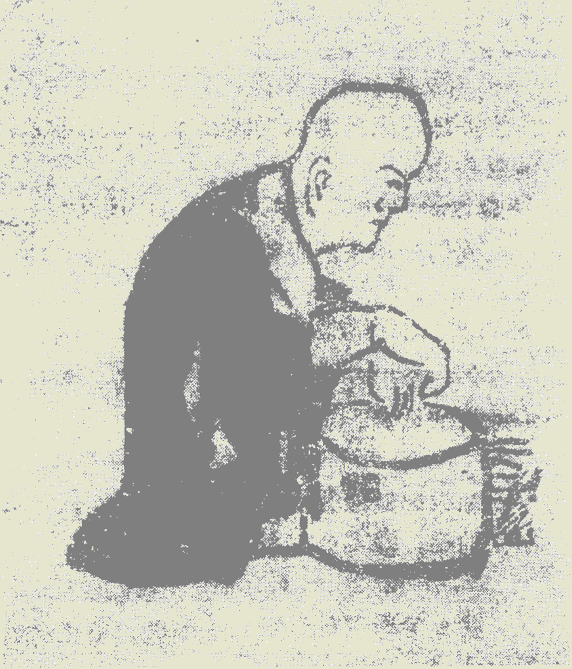
\includegraphics[height=0.9\textheight]{yosa}\\[1em]
        \large{\FS 与谢芜村自画像}
    \end{figure}
\end{center}

\newpage

{\FS
    与谢芜村(1716—1783),本姓谷口,名长庚,字春星,别号宰鸟、夜半翁等。生于摄津国东域郡毛马村(现大阪市都岛区毛马町)富裕的农家。二十岁起,就学俳谐,同时也学绘画。二十九岁时,用「芜村」名(来自陶渊明《归去来辞》的「田园将芜」)。编撰的著作有《玉藻集》、《夜半乐》、《新花摘》等。后期关于俳谐的奥义,曾对他的门人答问说:「用俗语而离俗好,离俗而用俗,离俗法最高。」这与芭蕉的「高悟心而归俗」是相通的。他所谓离俗,是离名利之地,「啸月赏花,游于尘寰之外。」又说「舍风雅而得风雅」,「得句贵在自然」。这些见解是高超的。

    芜村是俳人,也是画家(画南画,笔名子汉,四明,谢寅等)。句中有画,画中有句,崇尚王维。他的俳句,显出浓淡相宜的色彩美,又奇妙地把幻想世界具体化。著名俳人正冈子规对他有很高的评价。他有汉诗的修养,在其名作《春风马堤》\footnotemark[1] 十八首里面,四首用汉诗五言绝句体,所作俳句,也多带有汉诗的格调。作家上田秋成说他是用假名写汉诗的诗人,指出了他的作品的特点。我们可以看到他的诗,有中国的古典作品情趣。

    看来芜村的精神状态,较为乐观畅达,俳句的意境宽阔,而且潇洒华丽,富有浪漫主义色彩,与芭蕉的清寂、细致、质朴无华的现实主义风格,有所差别。他对芭蕉很崇敬,为的是着眼于复兴和提高俳句的艺术性。
}
\footnotetext[1]{\FS 此作乃是寄托归乡途中的女子,怀念久别母亲的心情。}

\newpage

\section{\FK 春}

\setcounter{haikucounter}{0}

\begin{haiku}
    {\FH \ruby[g]{公達}{きんだち}に、\ruby[g]{狐}{きつね}化けたり、\ruby[g]{宵}{よい}の春。}

    {\FK 狐狸变作公子身,灯夜乐游春。}

    {\FT 注:这是怪异俳句。}
\end{haiku}

\begin{haiku}
    {\FH 春の暮、家路に遠き、人ばかり。}

    {\FK 春日黄昏时,尽是远别归家人。}

    {\FT 注:诗人萩原朔太郎说芜村是个乡愁诗人。他写了不少怀乡俳句。}
\end{haiku}

\begin{haiku}
    {\FH ゆく春や、\ruby[g]{逡}{しゆん}\ruby[g]{巡}{じゆん}として、遅ざくら。}

    {\FK 暮春}

    {\FK 春将归去,樱花逡巡而开迟。}

    {\FT 注:原作「逡巡」用汉语。}
\end{haiku}

\begin{haiku}
    {\FH ゆく春や、横河へのぼる、いもの神。}

    {\FK 春将终,天花神,向横河塔攀登。}

    {\FT 注:江户时代,天花流行。母亲们为心爱的儿女担忧。横河塔为比睿山三塔之一。}
\end{haiku}

\begin{haiku}
    {\FH 春\ruby[g]{雨}{さめ}や、\ruby[g]{同車}{どうしゃ}の君が、さざめごと。}

    {\FK 春将归去,与汝同车,低声细语。}

    {\FT 注:汝是女性,典出《史记·孔子世家》卫灵公与夫人同车。}
\end{haiku}

\begin{haiku}
    {\FH \ruby[g]{瀟湘}{しょうしょう}の、雁のなみだや、\ruby[g]{朧}{おぼろ}月。}

    {\FK 春夜闻琴}

    {\FK 潇湘雁落泪,朦胧月色微。}

    {\FT 注:题意出自钱起《归雁》诗:「潇湘何事等闲回?水碧沙明两岸苔。二十五弦弹夜月,不胜清怨却飞来。」}
\end{haiku}

\begin{haiku}
    {\FH 女\ruby[g]{倶}{ぐ}して、\ruby[g]{内裏}{だいり}\ruby[g]{拝}{おが}まん、おぼろ月。}

    {\FK 朦胧月伴美女,同去瞻仰皇居。}

    {\FT 注:写春月的朦胧美,以及艳丽的美女和豪华的皇居。}
\end{haiku}

\begin{haiku}
    {\FH ぬはな\ruby[g]{生}{お}ふ、池の水かさや、春の雨。}

    {\FK 莼菜浮池面,春雨点点。}
\end{haiku}

\begin{haiku}
    {\FH 春雨や、小\ruby[g]{磯}{いそ}の小貝、ぬるるほど。}

    {\FK 春雨细细落,润湿沙滩小贝壳。}
\end{haiku}

\begin{haiku}
    {\FH 滝口に、燈を呼ぶ声や、春の雨。}

    {\FK 春夜雨濛濛,泷口所中,连呼快点灯。}

    {\FT 注:泷口在清凉殿东北,是宫中护卫武士值班所在,这表示发生了什么事故的不安感。}
\end{haiku}

\begin{haiku}
    {\FH 春雨や、ものかたりゆく、蓑と笠。}

    {\FK 春雨里,步行作恳谈,蓑与伞。}

    {\FT 注:蓑指农夫,伞指城市女人,二种身份,竟在春雨中边走边谈,饶有俳画情趣。}
\end{haiku}

\begin{haiku}
    {\FH \ruby[g]{高}{こ}\ruby[g]{麗}{ま}\ruby[g]{舟}{ぶね}の、よらで過ゆく、霞かな。}

    {\FK 高丽船,不靠岸,驶向彩霞天。}
\end{haiku}

\begin{haiku}
    {\FH 指南車を、\ruby[g]{胡}{こ}地に\ruby[g]{引}{ひき}\ruby[g]{去}{さ}る、霞哉。}

    {\FK 指南车入胡地,霞霭里,渐远去。}

    {\FT 注:指南车,中国古代指示方向的车,随后有长驱的大军。《宋史·舆服志》有记载。这句富有异国情调。}
\end{haiku}

\begin{haiku}
    {\FH 春の水、山なき国を、流れけり。}

    {\FK 春水流荡大平原。}

    {\FT 注:此句境界宽阔,气势雄伟。}
\end{haiku}

\begin{haiku}
    {\FH 春の海、\ruby[g]{終日}{ひねもす}のたり、のたり哉。}

    {\FK 春之海,整天荡去漂来。}

    {\FT 注:表示翻复单调的意思,这名句有淡远味。}
\end{haiku}

\begin{haiku}
    {\FH \ruby[g]{藪}{やぶ}入の、夢や\ruby[g]{小豆}{あづき}の、煮えるうち。}

    {\FK 年假省亲梦,就在小豆炊煮中。}

    {\FT 注:此作有《邯郸梦》的味道。}
\end{haiku}

\begin{haiku}
    {\FH \ruby[g]{雉}{きじ}啼や、草の武蔵の、八平氏。}

    {\FK 雉鸟声声啼,武藏野原深草地。想见八平氏。}

    {\FT 注:武藏八平氏,乃武威赫赫的豪族,也不过是一场繁华梦。这和芭蕉的俳句:「长夏草木深,武士当年梦痕」有一样的感慨。}
\end{haiku}

\begin{haiku}
    {\FH 歸る雁、田ごとの月の、曇る夜に。}

    {\FK 归来雁,映田春月朦胧夜。}
\end{haiku}

\begin{haiku}
    {\FH よく聞けば、桶に音を鳴く、田\ruby[g]{螺}{にし}哉。}

    {\FK 若是细细听,桶里田螺有叫声。}
\end{haiku}

\begin{haiku}
    {\FH \ruby[g]{伏勢}{ふくぜい}の、\ruby[g]{錣}{しころ}にとまる、胡蝶かな。}

    {\FK 蝴蝶翩翩,栖息伏兵盔帘上。}

    {\FT 注:蝴蝶飞来,在春野草丛的伏兵头盔上停留。伏兵即伊势平家武士,典出《平家物语》。盔帘日语作「錣」字,即头盔遮住脖子左右和后面的部分。}
\end{haiku}

\begin{haiku}
    {\FH \ruby[g]{釣鐘}{つりがね}に、とまりてねむる、こてふ哉。}

    {\FK 黄蝶停息于吊钟,安然进入梦中。}
\end{haiku}

\begin{haiku}
    {\FH 舟よせて、塩魚買ふや、\ruby[g]{岸}{きし}の梅。}

    {\FK 泊船买盐鱼,梅开满江堤。}
\end{haiku}

\begin{haiku}
    {\FH 白梅に、明くる夜ばかりと、なりにけり。}

    {\FK 初春}

    {\FK 白梅正初开,破晓只为看花来。}

    {\FT 注:写晚年沉浸美的境界和平静清闲的心情,正如许有壬《寻梅》诗所云:「何以慰我衰?梅花秀发时。」这是芜村临终前所吟三句的最后一句。}
\end{haiku}

\begin{haiku}
    {\FH 梅\ruby[g]{遠近}{おちこ}、\ruby[g]{南}{みんなみ}すべく、北すべく。}

    {\FK 远近梅花灿烂,我往北又往南。}
\end{haiku}

\begin{haiku}
    {\FH 白梅や、墨\ruby[g]{芳}{かんば}しき、\ruby[g]{鴻臚館}{こうろくわん}。}

    {\FK 鸿胪馆,白梅翰墨香。}

    {\FT 注:写在鸿胪馆与唐使吟诗作文的交欢。}
\end{haiku}

\begin{haiku}
    {\FH 不二\ruby[g]{颪}{おろし}、十三州の、やなぎかな。}

    {\FK 富士山风飘,十三州里柳枝摇。}

    {\FT 注:十三州指望得见富士山的十三个州。}
\end{haiku}

\begin{haiku}
    {\FH 花の香や、嵯峨のともし火、消る時。}

    {\FK 题花}

    {\FK 嵯峨灯光消失时,犹闻香花气。}
\end{haiku}

\begin{haiku}
    {\FH \ruby[g]{祇}{ぎ}や\ruby[g]{鑑}{かん}や、髭に落花を、\ruby[g]{捻}{ひねり}けり。}

    {\FK 花下联句惜春}

    {\FK 宗祇、宗鉴,捻动须上落花瓣。}

    {\FT 注:宗祇是连歌师,其须有名,山崎宗鉴是俳谐创始人,著有《犬筑波集》。}
\end{haiku}

\begin{haiku}
    {\FH 木の下が、\ruby[g]{蹄}{ひづめ}のかぜや、散さくら。}

    {\FK 风入马蹄轻}

    {\FK 风入蹄轻,树下落樱。}

    {\FT 注:「风入马蹄轻」来自杜甫《房兵曹胡马》「风入四蹄轻」句。}
\end{haiku}

\begin{haiku}
    {\FH 菜の花や、風月は東に、日は西に。}

    {\FK 春景}

    {\FK 一片菜花黄,东有新月,西有夕阳。}

    {\FT 注:写四月菜花盛开的春景。东西的描写,据说来源自陶渊明的「白日沦西河,素月出东岭。遥遥万里辉,荡荡空中景。」}
\end{haiku}

\begin{haiku}
    {\FH 菜の花や、鯨もよらず、海暮ぬ。}

    {\FK 菜花黄似金,鲸鱼离岸不靠近,海上正黄昏。}
\end{haiku}

\section{\FK 夏}

\setcounter{haikucounter}{0}

\begin{haiku}
    {\FH さみだれや、大河を前に、家二軒。}

    {\FK 梅雨不停下,面对大河两户人家。}

    {\FT 注:作者关心百姓人家的生活。}
\end{haiku}

\begin{haiku}
    {\FH ゆふだちや、筆もかはかず、一千言。}

    {\FK 双林寺独吟千句}

    {\FK 骤雨笔酣畅,挥写一千言。}
\end{haiku}

\begin{haiku}
    {\FH 夕だちや、草葉をつかむ、むら雀。}

    {\FK 骤雨蓦然下,群雀猛抓草叶。}
\end{haiku}

\begin{haiku}
    {\FH 夜水とる、里人の声や、夏の月。}

    {\FK 暑天月下人声喧,村民引水入干田。}
\end{haiku}

\begin{haiku}
    {\FH ぬけがけの、浅瀬わたるや、夏の月。}

    {\FK 夏月在天,先骑渡浅滩。}
\end{haiku}

\begin{haiku}
    {\FH 遠浅に、\ruby[g]{兵}{つはもの}舟や、夏の月。}

    {\FK 兵船停海面,夏月挂中天。}

    {\FT 注:白天作战,夜间休息。海上的兵船和空中的月亮,光波交映。}
\end{haiku}

\begin{haiku}
    {\FH \ruby[g]{河童}{かはたろ}の、恋する宿や、夏の月。}

    {\FK 夏天月下,河童钟情人家。}

    {\FT 注:河童是传说中的水怪,嘴尖面如虎。}
\end{haiku}

\begin{haiku}
    {\FH \ruby[g]{揚州}{ようしゅう}の、津も見えそめて、雲の峯。}

    {\FK 初见扬州港,云峰立在天。}

    {\FT 注:这是想象遣唐使到达中国的情景。}
\end{haiku}

\begin{haiku}
    {\FH \ruby[g]{離}{さ}\ruby[g]{別}{ら}れたる、身を\ruby[g]{蹈込}{ふんごん}で、田植哉。}

    {\FK 此身被休离,还是下田插秧去。}

    {\FT 注:写不幸的农村妇女被休后,时值农忙,还是下田,用体力劳动排遣精神上的悲哀。}
\end{haiku}

\begin{haiku}
    {\FH 夕風や、水\ruby[g]{青鷺}{あおさぎ}の、\ruby[g]{脛}{はぎ}をうつ。}

    {\FK 晚风轻轻,波触青鹭胫。}
\end{haiku}

\begin{haiku}
    {\FH \ruby[g]{鮎}{あゆ}くれて、よらで過行、夜半の門。}

    {\FK 留赠我香鱼,夜半悄悄过门去。}

    {\FT 注:鲇,夏季淡水鱼,能吐香气,又名香鱼。钓鲇鱼人为芜村好友,只留赠鲇鱼,过门不入。}
\end{haiku}

\begin{haiku}
    {\FH \ruby[g]{鮒}{ふな}ずしや、\ruby[g]{彦根}{ひこね}が\ruby[g]{城}{しろ}に、雲かかる。}

    {\FK 鲫鱼寿司味好,云绕彦根城堡。}

    {\FT 注:鲫鱼肉发酵后有酸味,将其夹在米饭中的食品,称为鲫鱼寿司,是江州的名产。彦根城是在琵琶湖边山腹的井伊家的城堡。}
\end{haiku}

\begin{haiku}
    {\FH 蚊の声す、\ruby[g]{忍冬}{にんどう}の花の、散るたびに。}

    {\FK 蚊子声细细,正是忍冬花落时。}

    {\FT 注:忍冬,一种蔓草,夏天开花,花色从白变黄,也称金银花。}
\end{haiku}

\begin{haiku}
    {\FH 谷路、行人は小き、若葉哉。}

    {\FK 新叶繁茂,峡谷路上行人少。}
\end{haiku}

\begin{haiku}
    {\FH 浅間山、煙の中の、若葉かな。}

    {\FK 浅间山,弥漫烟中嫩叶鲜。}
\end{haiku}

\begin{haiku}
    {\FH 不二ひとつ、\ruby[g]{埋}{うづ}み残して、わかばかな。}

    {\FK 新绿叶丛淹没中,只余富士一孤峰。}
\end{haiku}

\begin{haiku}
    {\FH 牡丹散りて、打かさなりぬ、二三\ruby[g]{片}{ぺん}。}

    {\FK 牡丹花散,叠地两三片。}
\end{haiku}

\begin{haiku}
    {\FH \ruby[g]{金屏}{きんびょう}の、かくやくとして、牡丹哉。}

    {\FK 金屏风上,牡丹花灿烂。}
\end{haiku}

\begin{haiku}
    {\FH 山\ruby[g]{蟻}{あり}の、あからさま\ruby[g]{也}{なり}、白牡丹。}

    {\FK 一只黑蚂蚁,忽然爬上白牡丹。}

    {\FT 注:一黑一白,色彩鲜明。}
\end{haiku}

\begin{haiku}
    {\FH \ruby[g]{蟻}{ぎ}王宮、朱門を開く、牡丹哉。}

    {\FK 蚁塚}

    {\FK 蚁王宫,牡丹花发朱门红。}

    {\FT 注:取材自李公佐《南柯记》的典故,写出荣华梦景。}
\end{haiku}

\begin{haiku}
    {\FH \ruby[g]{閻王}{えんおう}の、口や牡丹を、\ruby[g]{吐}{ぬ}かんとす。}

    {\FK 波翻舌本吐红莲}

    {\FK 阎王舌片,吐成红牡丹。}

    {\FT 注:标题出典未详。据云《阿弥陀经》有「舌相生红莲」的句子。}
\end{haiku}

\begin{haiku}
    {\FH 花いばら、故郷の路に、似たる哉。}

    {\FK 登东皋}

    {\FK 蔷薇花开处处,恰似故乡路。}

    {\FT 注:作者读陶渊明《归去来兮辞》「登东皋而舒啸,临清流而赋诗」句涌起自己的怀乡情。皋是岸边。蔷薇花的枝干多刺。}
\end{haiku}

\begin{haiku}
    {\FH \ruby[g]{愁}{うれ}ひつつ、岡にのぼれば、花いばら。}

    {\FK 怀愁登古丘,山路野薇幽。}
\end{haiku}

\begin{haiku}
    {\FH 水深く、\ruby[g]{利鎌}{ききかま}鳴らす、眞\ruby[g]{菰}{こも}刈。}

    {\FK 深水割菰蒲,锐利镰刀声。}

    {\FT 注:写爽快的情景。}
\end{haiku}

\begin{haiku}
    {\FH 水桶に、うなづきあふや、\ruby[g]{瓜}{うり}\ruby[g]{茄子}{なすび}。}

    {\FK 香瓜和茄子,相会点头水桶里。}

    {\FT 注:指碰到熟人时的幽默句。}
\end{haiku}

\section{\FK 秋}

\setcounter{haikucounter}{0}

\begin{haiku}
    {\FH 身にしむや、\ruby[g]{亡妻}{なきつま}の\ruby[g]{櫛}{くし}を、\ruby[g]{閨}{ねや}に踏。}

    {\FK 踩了亡妻梳子,感到闺房凉意。}
\end{haiku}

\begin{haiku}
    {\FH 猿どのの、夜寒\ruby[g]{訪}{とひ}ゆく、兎かな。}

    {\FK 秋凉夜,野兔拜访猴爷。}

    {\FT 注:芜村山居,拟鸟羽僧正的鸟兽戏画图作句,富有童话味。}
\end{haiku}

\begin{haiku}
    {\FH 去年より、又さびしいぞ、秋の暮。}

    {\FK 老怀}

    {\FK 又比去年更寂寞,秋之暮。}
\end{haiku}

\begin{haiku}
    {\FH 山鳥の、枝踏みかゆる、夜長哉。}

    {\FK 山鸟踏枝来又去,漫漫长夜里。}
\end{haiku}

\begin{haiku}
    {\FH 月天心、\ruby[g]{貧}{まず}しき町を、通りけり。}

    {\FK 月到天心,人过穷市镇。}

    {\FT 注:北宋邵雍《清夜吟》有「月到天心处」句。穷市镇白天不清洁,夜来被月洗净,欣赏此夜月景。}
\end{haiku}

\begin{haiku}
    {\FH 五六\ruby[g]{升}{しょう}、\ruby[g]{芋}{いも}煮る坊の、月夜哉。}

    {\FK 和尚煮芋五六升,只为今宵赏月明。}

    {\FT 注:一日升,合营造库平制一点七四一升。此是冒充风雅的幽默句。}
\end{haiku}

\begin{haiku}
    {\FH 四五人に、月落ちかかる、おどり哉。}

    {\FK 明月已西沉,舞蹈还有四五人。}

    {\FT 注:盂兰盆节之夜,家家男女集合跳舞,此是看名画家英一蝶(1652—1724)风俗画有感而作。}
\end{haiku}

\begin{haiku}
    {\FH 唐人よ、此花過て、のちの月。}

    {\FK 唐代诗人哟,此花开后还有月。}

    {\FT 注:元稹诗句:「不是花中偏爱菊,此花开尽更无花。」此花指重阳的菊,月指旧历九月十三日夜的月。日人赏月有八月十五仲秋夜,还有九月十三夜。}
\end{haiku}

\begin{haiku}
    {\FH \ruby[g]{唐黍}{とうきび}の、おどろきやすし、秋の風。}

    {\FK 萧簌吹秋风,黍叶易惊动。}

    {\FT 注:此作有汉诗的情趣,南唐李中有「门巷凉秋至,高梧一叶惊」诗句。}
\end{haiku}

\begin{haiku}
    {\FH \ruby[g]{秋風}{しうふう}や、\ruby[g]{酒肆}{しゅし}に\ruby[g]{詩}{し}うたふ、\ruby[g]{漁者}{ぎょしゃ}\ruby[g]{樵者}{せうしゃ}。}

    {\FK 秋风寂寥,酒肆吟诗有渔樵。}
\end{haiku}

\begin{haiku}
    {\FH 鳥羽殿へ、五\ruby[g]{六騎}{ろっき}いそぐ、野分哉。}

    {\FK 落木风天,五六骑,奔向鸟羽殿。}

    {\FT 注:鸟羽殿是鸟羽天皇的离宫。此种情景,表示宫廷将有事变发生。}
\end{haiku}

\begin{haiku}
    {\FH 白露や、茨の\ruby[g]{刺}{はり}に、ひとつづつ。}

    {\FK 荆棘多刺芒,根根闪耀白露光。}
\end{haiku}

\begin{haiku}
    {\FH いなづまや、\ruby[g]{堅田}{かたた}泊りの、宵の空。}

    {\FK 旅宿坚田,电光闪夜天。}

    {\FT 注:坚田在琵琶湖西岸,秋天多电光。}
\end{haiku}

\begin{haiku}
    {\FH いな妻や、佐渡なつかしき、舟便り。}

    {\FK 闪电光中望佐渡,盼船上捎来消息。}
\end{haiku}

\begin{haiku}
    {\FH \ruby[g]{負}{まく}まじき、\ruby[g]{角力}{すまひ}を寝もの、がたり哉。}

    {\FK 角力竞赛输,床上怨内助。}

    {\FT 注:这是写角力者在床上对妻罗唆着他的摔法和不该输掉的道理。相扑到芜村时,在大阪、京都、江户(东京)专业力士定于七月比赛。故相扑成为秋的季语。}
\end{haiku}

\begin{haiku}
    {\FH 鹿寒し、角も身に添ふ、枯木哉。}

    {\FK 角如枯木鹿身寒。}
\end{haiku}

\begin{haiku}
    {\FH 一行の、雁や\ruby[g]{端}{は}山に、月を\ruby[g]{印}{しる}す。}

    {\FK 探题雁字}

    {\FK 雁一行,月印端山上。}
\end{haiku}

\begin{haiku}
    {\FH 釣\ruby[g]{上}{のぼ}し、\ruby[g]{鱸}{すずき}の\ruby[g]{巨}{きょ}口、玉や\ruby[g]{吐}{はく}。}

    {\FK 钓上一尾鲈,巨口吐珍珠。}
\end{haiku}

\begin{haiku}
    {\FH \ruby[g]{沙魚}{はぜ}釣の、小舟\ruby[g]{漕}{こ}ぐなる、窓の前。}

    {\FK 小船钓虾虎,凭窗见摇橹。}

    {\FT 注:虾虎栖在河海之间,秋后钓它。这是在大阪的大川口、隅田川的河口等处水亭上所见的景象。}
\end{haiku}

\begin{haiku}
    {\FH 柳散り、\ruby[g]{清}{し}水\ruby[g]{涸}{かれ}石、\ruby[g]{処々}{ところどころ}。}

    {\FK 柳丝落下水枯涸,河石处处出。}

    {\FT 注:作者爱读苏轼《后赤壁赋》,赏识「山高月小,水落石出」句,奥羽(陆奥、出羽合称,是日本东北六县地区)旅行,写三景并列。}
\end{haiku}

\begin{haiku}
    {\FH 白菊や、呉山の雪を、笠の下。}

    {\FK 旧笠盖菊图}

    {\FK 白菊有如吴山雪,开在草笠下。}

    {\FT 注:宋僧可士句「笠重吴天雪」,「吴天」也用「吴山」。}
\end{haiku}

\begin{haiku}
    {\FH 朝がほや、一輪深き、\ruby[g]{淵}{ふち}のいろ。}

    {\FK 涧水湛如蓝}

    {\FK 牵牛花,一朵深渊色。}

    {\FT 注:标题是宋僧《碧岩录》的句子。}
\end{haiku}

\begin{haiku}
    {\FH 山は暮れて、野は\ruby[g]{黄昏}{たそがれ}の、\ruby[g]{薄}{すすき}哉。}

    {\FK 远山暮霭罩,原野苍茫落日照,蒙蒙狗尾草。}

    {\FT 注:这是芜村名句,为着表现它的境界,试用五、七、五句调译出。}
\end{haiku}

\begin{haiku}
    {\FH 落穂\ruby[g]{拾}{ひろ}ひ、日あたる方へ、あゆみ行。}

    {\FK 对着秋阳,拾穗人步步拾去。}

    {\FT 注:这俳句,正如法国米勒的田园风景画。}
\end{haiku}

\begin{haiku}
    {\FH 秋の燈や、ゆかしき奈良の、道具\ruby[g]{市}{いち}。}

    {\FK 秋夜街灯,奈良可亲旧货市。}
\end{haiku}

\section{\FK 冬}

\setcounter{haikucounter}{0}

\begin{haiku}
    {\FH 水鳥も、見えぬ江わたる、寒さ哉。}

    {\FK 不见浮禽渡江寒。}
\end{haiku}

\begin{haiku}
    {\FH うぐひすの、啼や\ruby[g]{師走}{しわす}の、羅生門。}

    {\FK 莺啼岁暮罗生门。}

    {\FT 注:罗生门为平城京及平安京的正门。平安京的罗生门址在东寺西。这里表示王朝情调的寂静气氛。}
\end{haiku}

\begin{haiku}
    {\FH 寒月や、枯木の中の、竹三竿。}

    {\FK 冬夜月光寒,枯树中间竹三竿。}

    {\FT 注:荒凉的枯树中,还有三枝翠竹映着寒夜月光。}
\end{haiku}

\begin{haiku}
    {\FH 寒月や、\ruby[g]{衆}{しゅ}徒の群議の、過て後。}

    {\FK 寒月映山头,僧兵议战后。}

    {\FT 注:这写属于《太平记》、《平家物语》的世界,比睿山三井寺僧兵在议论明天战事之后。}
\end{haiku}

\begin{haiku}
    {\FH 初雪の、\ruby[g]{底}{そこ}を\ruby[g]{叩}{たたけ}ば、竹の月。}

    {\FK 初雪倾盆落,竹林月色薄。}
\end{haiku}

\begin{haiku}
    {\FH 古池に、\ruby[g]{草履}{ぞうり}沈みて、みぞれ哉。}

    {\FK 古池沉草鞋,雨雪飘飘下。}
\end{haiku}

\begin{haiku}
    {\FH 大雪と、成けり関の、\ruby[g]{鎖}{とざ}し\ruby[g]{時}{ごろ}。}

    {\FK 大雪不停止,关所之门掩闭时。}

    {\FT 注:关所之门为大雪所封闭的情景,使人如见广重的浮世绘。}
\end{haiku}

\begin{haiku}
    {\FH 宿かせと、刀\ruby[g]{投}{なげ}\ruby[g]{出}{だ}す、吹雪哉。}

    {\FK 风雪夜来人,拔刀喊借宿。}

    {\FT 注:写浪人无赖的形象,带有戏剧性。}
\end{haiku}

\begin{haiku}
    {\FH \ruby[g]{凩}{こがらし}や、何に世わたる、家五軒。}

    {\FK 寒风吹得紧,谋生之道何处寻?此地五家人。}

    {\FT 注:写实景,同情穷人。}
\end{haiku}

\begin{haiku}
    {\FH 木枯や、鐘に小石を、吹あてる。}

    {\FK 飕飕寒风,吹起小石碰了钟。}
\end{haiku}

\begin{haiku}
    {\FH 水鳥や、舟に菜を洗ふ、女\ruby[g]{有}{あり}。}

    {\FK 冬川小舟浮,有女洗菜蔬。}
\end{haiku}

\begin{haiku}
    {\FH \ruby[g]{松明}{まつ}ふりて、舟橋わたる、夜の霜。}

    {\FK 松明晃过舟桥,夜霜耀。}
\end{haiku}

\begin{haiku}
    {\FH \ruby[g]{蕭條}{しょうじょう}として、石に日の入、枯野かな。}

    {\FK 荒野萧条不堪,夕阳沉没山石间。}

    {\FT 注:班固有「原野萧条」句,杜甫《望野》诗有「不堪人事日萧条」句,据云为芜村用「萧条」的来源。}
\end{haiku}

\begin{haiku}
    {\FH \ruby[g]{桃源}{とうげん}の、\ruby[g]{路次}{ろし}の細さよ、冬ごもり。}

    {\FK 题诗石上过荒野。}

    {\FK 冬天蛰居,正在桃源路深处。}
\end{haiku}

\begin{haiku}
    {\FH くすり\ruby[g]{喰}{ぐい}、人に\ruby[g]{語}{かた}るな、\ruby[g]{鹿ヶ}{ししが}谷。}

    {\FK 鹿谷吃药事,勿与人提起。}

    {\FT 注:鹿谷在京都左京区,大文字山的西麓。那里有俊宽僧都的山庄。治承元年(1177 年)藤原成亲、康赖等聚集商议讨伐平家而被捕。他们是以吃药食为名义到鹿谷的。药食是指平常嫌它不干净的鹿肉猪肉,冬寒时以为吃了能滋补身体。}
\end{haiku}

\begin{haiku}
    {\FH 枇杷の花、鳥もすさめず、日くれたり。}

    {\FK 日暮枇杷花儿艳,难与鸟儿消遣。}
\end{haiku}

\begin{haiku}
    {\FH \ruby[g]{寒梅}{かんばい}を、手折響や、老が\ruby[g]{肘}{ひじ}。}

    {\FK 寒梅折枝响,联想老胳臂。}

    {\FT 注:把寒瘠的梅枝与老瘦的胳臂作比。}
\end{haiku}

\begin{haiku}
    {\FH 斧入て、香におどろくや、冬\ruby[g]{木立}{こだち}。}

    {\FK 举斧砍枯木,惊异吐香气。}
\end{haiku}

\begin{haiku}
    {\FH 水仙に、狐遊ぶや、宵月夜。}

    {\FK 古丘}

    {\FK 狐狸取乐水仙旁,清冷月夜光。}

    {\FT 注:这是怪异俳句。}
\end{haiku}

\begin{haiku}
    {\FH \ruby[g]{葱}{ねぎ}\ruby[g]{買}{かう}て、枯木の中を、帰りけり。}

    {\FK 买了一把葱,枯林归路中。}

    {\FT 注:冬天菜蔬极少,能够买到新鲜青葱,心情愉快,通过枯木林路回家。青葱与枯木做对比。}
\end{haiku}

\begin{haiku}
    {\FH 我も死して、\ruby[g]{碑}{ひ}に\ruby[g]{辺}{ほとり}せむ、枯尾花。}

    {\FK 芭蕉翁墓前}

    {\FK 我死葬墓旁,亦愿作枯芒。}

    {\FT 注:在京都金福寺谒芭蕉墓后述怀之作。}
\end{haiku}

\chapter[{\FM 小林一茶}]{\FM \ruby[g]{小林}{こばやし}\ruby[g]{一茶}{いっさ}}

\begin{center}
    \begin{figure}
        \centering
        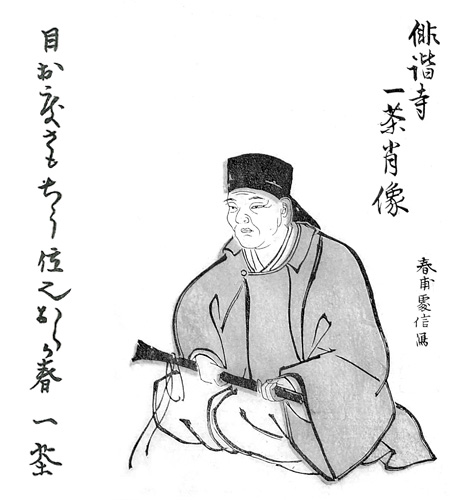
\includegraphics[width=\textwidth]{kobayashi}\\[1em]
        \large{\FS 小林一茶}
    \end{figure}
\end{center}

\newpage

{\FS
    小林一茶(1763—1827),本名弥太郎,生于信浓国水内郡柏原村(今长野县上水内郡信浓町柏原)农民家,三岁母亲去世,八岁来了继母,十岁有了异母弟,他受了虐待。廿五岁到江户,拜二六庵竹阿为师,开始学写俳谐。随后过着流浪生活,离开江户,从京都、大阪赴四国、九州旅行。后来往还于江户与故乡之间。他五十二岁才结婚,所生的三个男孩和一个女孩,均早夭折。六十一岁时,妻死去。六十二岁再娶,不到三个月离婚。六十四岁第三次结婚,留下遗腹女。家乡柏原大火,一茶的家也给烧光,他只好居住在幸存的贮藏室里面。这一年冬天,一茶就在这贮藏室里面逝世。

    一茶的俳句,由于他自己的经历,而形成了他自己的风格。他不大吟风弄月,只吟咏自己及其周围的平凡而不幸的生活,写庄重的句,也写幽默的句,总含点苦味。有人评论一茶,说「自嘲自笑,不是乐天,不是厌世,逸气超然。」他也抒写怀乡之情,他对故乡既有怀念,也有嫌恶的两种感情。他自我暴露,表示卑下无力,但也抒写不平事,却常用幽默和讽刺的手法。他特别慈爱,反对强者,同情弱者,喜爱小动物,对它们好像是好朋友一般亲切。我推测也许和他可悲的童年有关,他得不到家庭的温暖,就亲近乡间的小动物,成为物我一体。这在后来的俳句中充分表现出来。

    另一个是用语的特点,常运用俗语、方言、拟态语、拟声语等,看来像素描画一样。他的学生模仿他的俳风,他却告诫学生说,「我的俳风不可学。」其实没有他的素养和生活感受,也是学不来的。
}

\newpage

\section{\FK 新年}

\setcounter{haikucounter}{0}

\begin{haiku}
    {\FH 元日や、我のみならぬ、巣なし鳥。}

    {\FK 元旦寂寥,不止我是无巢鸟。}
\end{haiku}

\begin{haiku}
    {\FH 元日や、上々\ruby[g]{吉}{きち}の、浅\ruby[g]{黄}{ぎ}空。}

    {\FK 元旦日,大吉大利,浅黄晴空色。}
\end{haiku}

\begin{haiku}
    {\FH \ruby[g]{這}{は}へ笑へ、二つになるぞ、けさからは。}

    {\FK 对两岁的小孩说}

    {\FK 爬吧,笑吧,从今朝起两岁啦!}
\end{haiku}

\begin{haiku}
    {\FH 藪入や、墓の松風、うしろ吹。}

    {\FK 假日回家,坟墓松风身后吹。}

    {\FT 注:假日回家,指男女佣人每年于正月和七月的十六日放假回家。}
\end{haiku}

\begin{haiku}
    {\FH \ruby[g]{逃}{のが}しなや、水祝はるゝ、五十\ruby[g]{聟}{むこ}。}

    {\FK 别让他逃开,被水祝的半百新郎。}

    {\FT 注:水祝,新年亲友到前年结婚的男方家里,泼水祝贺。}
\end{haiku}

\begin{haiku}
    {\FH 舞\ruby[g]{扇}{おうぎ}、猿の涙の、かゝる哉。}

    {\FK 猴子泪水湿舞扇。}

    {\FT 注:作者同情被迫卖艺的猴子。}
\end{haiku}

\begin{haiku}
    {\FH \ruby[g]{垢爪}{あかつめ}や、\ruby[g]{薺}{なずな}の前も、はづかしき。}

    {\FK 人日}

    {\FK 不干净的指甲,在荠菜前,也感到羞惭啊!}

    {\FT 注:人日,中国古时从元旦到正月八日,分为鸡、狗、猪、羊、牛、马、人、谷的日子。正月七日为人日。荠菜,十字花科,春日开花,花小色白,它的嫩茎嫩叶,可供食用,《诗经·邶风·谷风》,有「其甘如荠」句。日本旧俗在人日吃七草粥,内有荠、芹、母子草、佛座、繁缕、芜菁、萝卜七种,以为可除百病,《荆楚岁时记》有记载。荠在人日是吉祥物,指甲沾着荠汁而切荠菜,被认为不干净,故对荠有羞惭之意。\footnote{\FT 日本「春の七草」,用来制作「七草粥」的七种植物,分别是:水芹(芹,せり)、荠菜(荠,なずな)、鼠曲草(古称:御形,ごぎょう;今名:母子草,ははこぐさ)、繁缕(繁缕,古音:はこべら,今音:はこべ),稻槎菜(古名:仏の座,ほとけのざ;今名:小鬼田平子,こおにたびらこ)、芜菁(古名:菘,すずな:今名:芜,かぶ)、萝卜(古名:萝卜,すずしろ;今名:大根,だいこん)。}}
\end{haiku}

\section{\FK 春}

\setcounter{haikucounter}{0}

\begin{haiku}
    {\FH 春雨や、\ruby[g]{喰}{くわ}れ残りの、鴨が鳴。}

    {\FK 春雨纷纷落,吃剩的鸭子叫着。}

    {\FT 注:冬天捕到的野鸭,大多已经吃掉,有的留到春来时还在叫着,被认为是吃剩的。}
\end{haiku}

\begin{haiku}
    {\FH 春めくや、藪ありて雪、ありて雪。}

    {\FK 春意温和,竹林还有积雪,还有积雪。}
\end{haiku}

\begin{haiku}
    {\FH 三\ruby[g]{文}{もん}が、霞見にけり、遠眼鏡。}

    {\FK 白日登汤台}

    {\FK 三文钱租望远镜,望望春霞景。}

    {\FT 注:白日登汤岛天神境内的高台。}
\end{haiku}

\begin{haiku}
    {\FH 西山や、おのれがのるは、どのかすみ。}

    {\FK 西山啊!哪朵云霞乘了我?}

    {\FT 注:经由专明寺主持调停,一茶与异母弟仙六取得和解。于一八一三年春(五十岁)定居故乡,作此喜悦的幽默句。}
\end{haiku}

\begin{haiku}
    {\FH 横乗の、馬のつゞくや、夕がすみ。}

    {\FK 晚霞里,横骑马儿何处去?}

    {\FT 注:写农民忙了一天,在晚霞下,横坐马背上归家。}
\end{haiku}

\begin{haiku}
    {\FH かすむ日や、夕山かげの、\ruby[g]{飴}{あめ}の笛。}

    {\FK 暮色苍茫,山那方,吹笛卖饴糖。}
\end{haiku}

\begin{haiku}
    {\FH \ruby[g]{我庵}{わがいお}や、貧乏がくしの、雪とける。}

    {\FK 掩盖我贫家的雪,已经融解。}

    {\FT 注:信浓雪大,一片白茫茫的雪,盖着房屋,分不清谁是富家,谁是穷家。}
\end{haiku}

\begin{haiku}
    {\FH \ruby[g]{米}{こめ}\ruby[g]{蒔}{ま}くも、罪ぞよ鶏が、けあふぞよ。}

    {\FK 撒把米也是罪过啊!让鸡斗起来。}

    {\FT 注:此句富有理趣,无季语。}
\end{haiku}

\begin{haiku}
    {\FH 亡き母や、海見る\ruby[g]{度}{たび}に、見るたびに。}

    {\FK 想念去世的母亲,当看到海时,看到海时。}

    {\FT 注:五十岁时春三月到千叶富津后,看到大海,感叹自己的流浪,便怀念去世的母亲。此句无季语。}
\end{haiku}

\begin{haiku}
    {\FH 春日のや、あくたれ鹿も、\ruby[g]{角}{つの}落る。}

    {\FK 春日野,鹿角给恶作剧地锯掉。}

    {\FT 注:鹿是奈良春日野神的使者,每年春因防伤人被锯掉。}
\end{haiku}

\begin{haiku}
    {\FH 其夜から、雨に\ruby[g]{逢}{あい}けり、巣立鳥。}

    {\FK 出巢鸟从那一夜起,就碰到落雨。}
\end{haiku}

\begin{haiku}
    {\FH 雀の子、そこのけそこのけ、\ruby[g]{御馬}{おんま}が通る。}

    {\FK 小麻雀,躲开,躲开,马儿就要过来。}
\end{haiku}

\begin{haiku}
    {\FH 我と来て、あそぶや親の、ない雀。}

    {\FK 到我这里来玩哟!没有爹娘的麻雀。}

    {\FT 注:一茶三岁时母亲去世,这是回忆六岁时的吟句,一茶的代表作之一。我觉得文言的译法「孤雀勿哀,与我嬉来」不如用白话表现得更情真意切。}
\end{haiku}

\begin{haiku}
    {\FH 夕燕、我には翌の、あてはなき。}

    {\FK 黄昏燕子有归巢,我没有明天的目标。}

    {\FT 注:这是一茶四十五岁时作,那时居无定所,辗转于上总、下总、常陆之间,故有此感慨。}
\end{haiku}

\begin{haiku}
    {\FH 柳さす、我をさみする、烏哉。}

    {\FK 绿柳枝斜,漠然栖着一乌鸦。}
\end{haiku}

\begin{haiku}
    {\FH \ruby[g]{近江}{おうみ}のや、雁のかへりも、松の月。}

    {\FK 近江归雁松月明。}
\end{haiku}

\begin{haiku}
    {\FH 帰雁、浅間のけぶり、いく度見る。}

    {\FK 归来的雁,见过几回浅间山云烟?}
\end{haiku}

\begin{haiku}
    {\FH \ruby[g]{痩蛙}{やせがえる}、まけるな一茶、\ruby[g]{是}{これ}に有り。}

    {\FK 观斗蛙,四月二十日}

    {\FK 瘦青蛙,别输掉,这里有我一茶!}

    {\FT 注:旧时有斗蛙的习俗。一茶于武藏国(今东京都足立区)竹冢看斗蛙,表示支援弱者。这是一茶的代表作之一。}
\end{haiku}

\begin{haiku}
    {\FH \ruby[g]{悠然}{ゆうぜん}として、山を見る、蛙哉。}

    {\FK 青蛙悠然见南山。}

    {\FT 注:「悠然」是原作用汉语的词儿。}
\end{haiku}

\begin{haiku}
    {\FH とぶ蝶の、人をうるさく、思ふらめ。}

    {\FK 蝴蝶飞远,似不企望这人间。}
\end{haiku}

\begin{haiku}
    {\FH 人\ruby[g]{並}{なみ}に、棚の\ruby[g]{蚕}{かいこ}も、昼寝哉。}

    {\FK 像人一样,棚里的蚕也午睡了。}
\end{haiku}

\begin{haiku}
    {\FH 夕月や、鍋の中にて、鳴田にし。}

    {\FK 黄昏月升时,田螺在锅里啼泣。}
\end{haiku}

\begin{haiku}
    {\FH \ruby[g]{蛤}{はまぐり}の、\ruby[g]{芥}{ごみ}を\ruby[g]{吐}{はか}する、月夜かな。}

    {\FK 月夜里,蚌吐泥。}
\end{haiku}

\begin{haiku}
    {\FH おらが世や、そこらの草も、餅になる。}

    {\FK 生我故乡地,那儿的草,可以做饼哩!}
\end{haiku}

\begin{haiku}
    {\FH 餅になる、草が青むぞ、青むぞよ。}

    {\FK 做饼的草,长青了哩,长青了哩!}

    {\FT 注:可以看到天真的童心,发出惊奇的声调。}
\end{haiku}

\begin{haiku}
    {\FH 梅\ruby[g]{一枝}{ひとえ}、とる人を待、ゆふべ哉。}

    {\FK 黄昏时,等待折梅一枝的人儿。}
\end{haiku}

\begin{haiku}
    {\FH 梅がゝや、どなたが来ても、\ruby[g]{欠}{かけ}茶碗。}

    {\FK 人家去赏香梅,我却谁来也是破茶杯。}
\end{haiku}

\begin{haiku}
    {\FH ゆうゆうと、茨のおくの、野梅哉。}

    {\FK 野薇丛里,野梅悠然开。}
\end{haiku}

\begin{haiku}
    {\FH 茶の煙、柳と共に、そよぐ\ruby[g]{也}{なり}。}

    {\FK 柳枝与茶烟,随风荡漾。}
\end{haiku}

\section{\FK 夏}

\setcounter{haikucounter}{0}

\begin{haiku}
    {\FH 大の字に、寝て涼しさよ、淋しさよ。}

    {\FK 像「大」字一样躺着,又凉爽又无聊。}
\end{haiku}

\begin{haiku}
    {\FH 涼風の、\ruby[g]{曲}{まが}りくねって、来たりけり。}

    {\FK 住里屋}

    {\FK 凉风吹进来,曲折而迂回。}
\end{haiku}

\begin{haiku}
    {\FH \ruby[g]{帰去来}{いざいなん}、江戸は涼みも、むつかしき。}

    {\FK 回家去吧,江户乘凉也难呀!}
\end{haiku}

\begin{haiku}
    {\FH 涼風に、月をも添て、五文哉。}

    {\FK 清风加朗月,五文钱。}

    {\FT 注:是从李白《襄阳歌》「清风朗月不用一钱买」变化来的,李白不用一钱买,一茶却给五文钱。}
\end{haiku}

\begin{haiku}
    {\FH 橋涼し、張良たのむ、此\ruby[g]{沓}{くつ}を。}

    {\FK 桥上凉风吹,张良捡取这鞋来。}

    {\FT 注:典出黄石公在圯上叫张良取鞋的故事。李白有诗《经下邳圯桥怀张子房》。}
\end{haiku}

\begin{haiku}
    {\FH 涼風の、\ruby[g]{浄土}{じょうど}\ruby[g]{則}{すなはち}、我家哉。}

    {\FK 风凉的净土,就是我的房屋。}
\end{haiku}

\begin{haiku}
    {\FH もたいなや、昼寝して聞、田うへ唄。}

    {\FK 粒粒皆辛苦}

    {\FK 万不该啊!午睡时,听唱插秧歌。}

    {\FT 注:标题引用唐李绅《古风》诗句。}
\end{haiku}

\begin{haiku}
    {\FH 五十\ruby[g]{聟}{むこ}、\ruby[g]{天窓}{あたま}をかくす、扇かな。}

    {\FK 五十做新郎,白发扇遮挡。}

    {\FT 注:一茶做新郎时,实是五十二岁,娶二十八岁的菊女为妻。扇为婚礼用品。此作是自我嘲弄。}
\end{haiku}

\begin{haiku}
    {\FH 寝せつけし、子のせんたくや、夏の月。}

    {\FK 孩子已入眠,离屋为他洗尿片,夏月挂天边。}
\end{haiku}

\begin{haiku}
    {\FH 湖水から、\ruby[g]{出現}{しゅつげん}したり、雲の峯。}

    {\FK 真谧静,湖水底下云峰影。}
\end{haiku}

\begin{haiku}
    {\FH \ruby[g]{蝸牛}{かたつむり}、ともども不二へ、上る\ruby[g]{也}{なり}。}

    {\FK 蜗牛一块儿,爬上富士山去也。}

    {\FT 注:写小动物与大高山的对照。比喻集体团结,去完成理想的力量。}
\end{haiku}

\begin{haiku}
    {\FH はらはらと、汗の玉ちる、稲葉哉。}

    {\FK 哗啦哗啦地,汗珠滴落的稻叶。}
\end{haiku}

\begin{haiku}
    {\FH 白雲を、\ruby[g]{袂}{たもと}に入て、\ruby[g]{袷}{あわせ}かな。}

    {\FK 夹袄两袖装白云。}

    {\FT 注:这句从「两袖清风」转化过来的,更饶情趣。}
\end{haiku}

\begin{haiku}
    {\FH 鹿の背に、くすくす鳥の、昼寝哉。}

    {\FK 在奈良}

    {\FK 鹿背上,笑嬉嬉的鸟儿,午睡入梦乡了。}
\end{haiku}

\begin{haiku}
    {\FH 時鳥、何を忘て、引返す。}

    {\FK 布谷鸟,忘记了什么,又转回来?}
\end{haiku}

\begin{haiku}
    {\FH 江戸へいざ、江戸へいざと、時鳥。}

    {\FK 足下也到江户去么?布谷鸟。}
\end{haiku}

\begin{haiku}
    {\FH 前の世の、おれがいとこか、\ruby[g]{閑古鳥}{かんこどり}。}

    {\FK 前生我们是堂兄弟么?布谷鸟。}
\end{haiku}

\begin{haiku}
    {\FH 鳰の巣の、一本草を、たのみ哉。}

    {\FK 䴙䴘的巢,全靠一根草。}

    {\FT 注:巢用芦苇梢端拗折交错而成,浮在水面,也有用零碎的芦苇做成,把巢系在杂草或灯芯草的茎上。}
\end{haiku}

\begin{haiku}
    {\FH 娘見よ、身を\ruby[g]{売}{うら}れつゝ、行蛍。}

    {\FK 女儿看啊,正被卖身去的萤火虫。}

    {\FT 注:夏天有钱人买萤火虫,装在纱袋里,悬在室内,或放在院子里飞翔,以供玩乐。}
\end{haiku}

\begin{haiku}
    {\FH けふの日も、\ruby[g]{棒}{ぼう}ふり虫よ、翌も又。}

    {\FK 日日懈怠,不惜寸阴}

    {\FK 今天是这样,像孑孓游游荡荡,明天也这样。}

    {\FT 注:题用汉文。孑孓是蚊的幼虫。}
\end{haiku}

\begin{haiku}
    {\FH 昼の蚊を、後にかくす、仏かな。}

    {\FK 佛陀将白天的蚊虫,藏在背后。}
\end{haiku}

\begin{haiku}
    {\FH 古郷は、蠅すら人を、さしにけり。}

    {\FK 心所思}

    {\FK 故乡哟,连苍蝇也螫人。}
\end{haiku}

\begin{haiku}
    {\FH やれ打な、蠅が手をすり、足をする。}

    {\FK 别拍打呀,苍蝇手揖脚跪啦!}
\end{haiku}

\begin{haiku}
    {\FH \ruby[g]{蚤}{のみ}の迹、かぞへながらに、添\ruby[g]{乳}{ぢ}哉。}

    {\FK 在喂奶时,又数跳蚤的痕迹。}
\end{haiku}

\begin{haiku}
    {\FH やけ土の、ほかりほかりや、蚤さわぐ。}

    {\FK 火烧场,跳蚤哄哄地乱嚷。}
\end{haiku}

\begin{haiku}
    {\FH 蝉鳴や、空にひつゝく、最上川。}

    {\FK 最上川,蝉声贴在天。}
\end{haiku}

\begin{haiku}
    {\FH 朝やけが、よろこばしいか、蝸牛。}

    {\FK 朝霞红艳艳,蜗牛啊,你可喜欢?}
\end{haiku}

\begin{haiku}
    {\FH 麦秋や、子を\ruby[g]{負}{おひ}ながら、いはし売。}

    {\FK 哀旅贩越后女}

    {\FK 麦秋时节,背着孩子,外出贩卖沙丁鱼。}

    {\FT 注:写越后(今新潟县)妇女的艰苦生活,沙丁鱼是用盐腌的。}
\end{haiku}

\begin{haiku}
    {\FH \ruby[g]{蕗}{ふき}の葉に、いはしを\ruby[g]{配}{くば}る、田植哉。}

    {\FK 每人发一份,款冬叶包沙丁鱼,插秧农忙时。}

    {\FT 注:款冬叶包沙丁鱼,写农村生活的情趣。农忙时,每人分发一份表示慰劳。}
\end{haiku}

\begin{haiku}
    {\FH 初瓜を、引とらまいて、寝た子哉。}

    {\FK 抓着新熟的瓜,睡着的孩子。}
\end{haiku}

\begin{haiku}
    {\FH 塔ばかり、見へて東寺は、夏木立。}

    {\FK 只见五重塔,东寺夏荫遮。}
\end{haiku}

\begin{haiku}
    {\FH 古郷や、よるも\ruby[g]{障}{さは}るも、\ruby[g]{茨}{ばら}の花。}

    {\FK 故乡呀,挨着碰着,都是带刺的花。}
\end{haiku}

\begin{haiku}
    {\FH 昼顔や、ぽっぽと燃る、石ころへ。}

    {\FK 烧热岩石中,旋花欣向荣。}

    {\FT 注:炎夏访喷火后的浅间山麓,赞扬小小花草的生命力。旋花为野生植物,初夏起开淡红色的花,状如牵牛花,午间时盛开,故在日本称昼颜。}
\end{haiku}

\section{\FK 秋}

\setcounter{haikucounter}{0}

\begin{haiku}
    {\FH 秋立や、身はならはしの、よ\ruby[g]{所}{そ}の窓。}

    {\FK 立秋了,站惯别人的窗口外。}
\end{haiku}

\begin{haiku}
    {\FH うそ寒や、\ruby[g]{蚯蚓}{みみず}の唄も、一夜づゝ。}

    {\FK 微寒夜夜里,蚯蚓在唱歌哩。}

    {\FT 注:蚯蚓无发音器官,但作者想象它会唱歌。}
\end{haiku}

\begin{haiku}
    {\FH 秋の夜や、旅の男の、針仕事。}

    {\FK 旅中秋夜里,男人做针线活。}

    {\FT 注:一茶漂泊三十六年,尤其是一七九五年的大旅行,当会有这生活的实感。}
\end{haiku}

\begin{haiku}
    {\FH 我星は、どこに旅寝や、天の川。}

    {\FK 我这颗星,何处寄宿啊?银河。}
\end{haiku}

\begin{haiku}
    {\FH 秋の夜や、窓の小穴が、笛を吹。}

    {\FK 秋夜间,纸窗小破口,吹起笛子响。}
\end{haiku}

\begin{haiku}
    {\FH うつくしや、せうじの穴の、天の川。}

    {\FK 病中}

    {\FK 多美啊!透过纸窗破洞看银河。}
\end{haiku}

\begin{haiku}
    {\FH 木曽山に、\ruby[g]{流}{ながれ}\ruby[g]{入}{いり}けり、天の川。}

    {\FK 银河倾泻木曾山。}

    {\FT 注:木曾山可能在一茶故乡信浓境内,指木曾诸山。木曾在今长野县西南部,木曾川上游山谷地乃桧木产地。此句写沉郁静美的夜空。}
\end{haiku}

\begin{haiku}
    {\FH 又人に、かけ\ruby[g]{抜}{ぬか}れけり、秋の暮。}

    {\FK 秋日黄昏行脚里,后面有人赶前去。}
\end{haiku}

\begin{haiku}
    {\FH たまに来た、古郷の月は、曇りけり。}

    {\FK 偶尔回家转,故乡的月色暗淡。}
\end{haiku}

\begin{haiku}
    {\FH 名月を、さしてかまはぬ、草家哉。}

    {\FK 如明月之所见,我的破家园。}
\end{haiku}

\begin{haiku}
    {\FH あの月を、とってくれろと、泣子哉。}

    {\FK 小孩哭着嚷,要取那月亮。}
\end{haiku}

\begin{haiku}
    {\FH 名月や、けふはあなたも、いそがしき。}

    {\FK 明月呀,今天你也贵忙。}

    {\FT 注:用「你」使人感觉亲切,想到月亮移行很快。}
\end{haiku}

\begin{haiku}
    {\FH \ruby[g]{義経}{よしつね}は、松の月さへ、ひいき哉。}

    {\FK 源义经,松月也对他表同情。}

    {\FT 注:源义经战功显赫,终为其兄源赖朝所不容,此句写出松月对义经也寄写同情。}
\end{haiku}

\begin{haiku}
    {\FH 同じ年の、顔の\ruby[g]{皺}{しわ}見ゆる、灯籠哉。}

    {\FK 灯笼啊,照见同年人的皱容。}
\end{haiku}

\begin{haiku}
    {\FH 案山子にも、うしろ向かれし、\ruby[g]{栖}{すみか}哉。}

    {\FK 我的家呀,稻草人也不理睬。}

    {\FT 注:写回乡后不顺心。稻草人是秋的季语。}
\end{haiku}

\begin{haiku}
    {\FH 馬の子の、故郷はなるゝ、秋の雨。}

    {\FK 秋雨绵绵,小马卖出离故乡。}
\end{haiku}

\begin{haiku}
    {\FH なくな雁、けふから我も、旅人ぞ。}

    {\FK 雁别叫了,从今天起,我也是漂泊者啊!}
\end{haiku}

\begin{haiku}
    {\FH 田の雁や、里の人数は、けふもへる。}

    {\FK 田里雁声叫,村中人见少。}

    {\FT 注:人见少,指信浓的旧俗,从晚秋到春天,壮年人出外谋生。}
\end{haiku}

\begin{haiku}
    {\FH 秋風に、歩行て逃る、蛍哉。}

    {\FK 萤火虫,步行潜逃避秋风。}

    {\FT 注:秋来了,萤火虫已经衰弱无力,以步行来表现它。作者自况。}
\end{haiku}

\begin{haiku}
    {\FH \ruby[g]{仰}{あう}のけに、寝て鳴にけり、秋の蝉。}

    {\FK 秋天的知了,仰卧地上向天叫。}
\end{haiku}

\begin{haiku}
    {\FH 秋風や、むしりたがりし、赤い花。}

    {\FK 长女莎托墓前}

    {\FK 秋风呀,小红花,要被撕碎了的!}

    {\FT 注:一茶的长女生于一八一八年五月四日,翌年患痘疮,于六月二十一日死。}
\end{haiku}

\begin{haiku}
    {\FH 蟷螂が、不二の\ruby[g]{麓}{ふもと}に、かゝる哉。}

    {\FK 螳螂爬到富士山麓。}
\end{haiku}

\begin{haiku}
    {\FH 人をとる、茸はたして、うつくしき。}

    {\FK 毒蘑菇}

    {\FK 害人的蘑菇,果然很娇妩。}
\end{haiku}

\begin{haiku}
    {\FH 夕暮に、むしろちれちれ、菊の花。}

    {\FK 夕阳落脚下,地上野菊花。}
\end{haiku}

\section{\FK 冬}

\setcounter{haikucounter}{0}

\begin{haiku}
    {\FH \ruby[g]{椋}{むく}鳥と、人に呼るゝ、寒哉。}

    {\FK 往东国途中}

    {\FK 人们呼唤白头翁,感到寒气重。}

    {\FT 注:东国指关东地区。信浓的白头翁鸟出现在寒冬时节。一茶五十岁时在《七番日记》中说自己是白头翁,这里人与鸟是相关的。}
\end{haiku}

\begin{haiku}
    {\FH 次の間の、灯で飯を喰ふ、夜寒哉。}

    {\FK 孤身旅行}

    {\FK 隔壁自进餐,灯暗风又寒。}
\end{haiku}

\begin{haiku}
    {\FH \ruby[g]{朝晴}{あさばれ}に、ぱちぱち\ruby[g]{炭}{すみ}の、きげん哉。}

    {\FK 早晨晴朗,火炭毕毕剥剥好舒畅。}
\end{haiku}

\begin{haiku}
    {\FH 行としや、空の青さに、守\ruby[g]{谷}{や}迄。}

    {\FK 廿三日入西林寺}

    {\FK 辞岁青空下,步行到守谷。}

    {\FT 注:一茶于一八一〇年十二月入守谷西林寺。守谷今茨城县北相马郡守谷町。}
\end{haiku}

\begin{haiku}
    {\FH 人並に、正月を待つ、灯影かな。}

    {\FK 像普通人,灯火期待新春。}
\end{haiku}

\begin{haiku}
    {\FH \ruby[g]{業}{ごう}の鳥、罠を巡るや、むら時雨。}

    {\FK 强盗藏在我的故乡被捕}

    {\FK 村间雨落,作孽的鸟,陷入圈套。}
\end{haiku}

\begin{haiku}
    {\FH しぐるゝや、芭蕉\ruby[g]{翁}{おきな}の、塚まはり。}

    {\FK 冬天的雨呀,绕着芭蕉翁的墓地。}
\end{haiku}

\begin{haiku}
    {\FH 木がらしや、\ruby[g]{地}{じ}びたに暮るゝ、辻\ruby[g]{諷}{うた}ひ。}

    {\FK 人生道路比山川还艰险}

    {\FK 寒风飘摇日将暮,有人卖唱十字路。}
\end{haiku}

\begin{haiku}
    {\FH 行人を、\ruby[g]{皿}{さら}でまねくや、薬喰。}

    {\FK 用碟子招呼行人,尝尝药食品。}

    {\FT 注:药食品是由鹿肉配药材煮成的。}
\end{haiku}

\begin{haiku}
    {\FH あゝまゝよ、年が暮よと、くれまいと。}

    {\FK 在此年关下,不管是好还是歹,任凭你安排。}
\end{haiku}

\begin{haiku}
    {\FH 心から、\ruby[g]{信濃}{しなの}の雪に、降られけり。}

    {\FK 信浓的雪,从心头落下。}

    {\FT 注:指家乡的人情淡薄,这里的雪成为袭击生活的东西,与风雅咏雪,全然异趣。}
\end{haiku}

\begin{haiku}
    {\FH うまさふな、雪やふふはり、ふふはりと。}

    {\FK 许是好吃的雪花,乱纷纷地飘下。}
\end{haiku}

\begin{haiku}
    {\FH 是がまあ、つひの栖か、雪五尺。}

    {\FK 十二月廿四日入故乡}

    {\FK 这终老住居地,哦,雪五尺!}

    {\FT 注:《八番日记》记每年要开支一笔扫雪费。一茶住这雪国,据统计写雪俳句有四百多首。此句是一八一二年(五十岁)写的。}
\end{haiku}

\begin{haiku}
    {\FH 真直な、小便穴や、門の雪。}

    {\FK 门前雪,小便洞真直}

    {\FT 注:这句有点卑俗,是生活的实感。蕉门其角也有这么个句子:「初雪里,这小便是哪个小子的?」}
\end{haiku}

\begin{haiku}
    {\FH 野仏の、御鼻の先の、\ruby[g]{氷柱}{つらら}哉。}

    {\FK 野佛鼻梁挂冰柱。}
\end{haiku}

\begin{haiku}
    {\FH 母親を、霜よけにして、寝た子哉。}

    {\FK 睡着的孩子,将母亲当防霜帘子}
\end{haiku}

\begin{haiku}
    {\FH 冬籠る、蛇の隣や、鼠穴。}

    {\FK 蛇蛰居过冬,邻家便是老鼠洞。}
\end{haiku}

\begin{haiku}
    {\FH \ruby[g]{象潟}{きさかた}の、欠をかぞへて、鳴千鳥。}

    {\FK 鸟海山埋海里,千满寺入地底}

    {\FK 象潟的千鸟,抓着破片啼叫。}

    {\FT 注:鸟海山,羽前羽后之间的名山,又称出羽富士。千满寺,即象潟的千满珠寺。千鸟是候鸟,嘴尖体小,背黑腹白,尾短腿长,冬天群集河、海上。千鸟,冬的季语。象潟曾于一八〇四年遭过地震,标题写出了地震的毁灭力。芭蕉《奥川小道》说游过此地。一茶不知何时到奥羽旅行,写下这真实的印象。}
\end{haiku}

\begin{haiku}
    {\FH 大根引、大根で道を、教へけり。}

    {\FK 拔萝卜的,拿着萝卜指路。}

    {\FT 注:写朴素的田园风景,活现指路人形象,还可想见有个问路人。}
\end{haiku}

\begin{haiku}
    {\FH \ruby[g]{焚}{た}くほどは、風がくれたる、おち葉哉。}

    {\FK 燃料够了,风送来的落叶。}

    {\FT 注:这是名作。}
\end{haiku}

\begin{haiku}
    {\FH こやし\ruby[g]{積}{つむ}、夕山\ruby[g]{畠}{ばた}や、散紅葉。}

    {\FK 粪肥堆叠,夕暮山田散红叶。}

    {\FT 注:红叶经晚秋、初冬的风雨而凋落,称散红叶或残红叶,属冬红叶一类。}
\end{haiku}

\begin{haiku}
    {\FH 家ありて、そして水仙、畠かな。}

    {\FK 有个家,再建个水仙园吧。}
\end{haiku}

\chapter[{\FS 寻钟声的余韵(代跋)}]{\FS 寻钟声的余韵(代跋)\\\hspace{2em}——俳句学习笔记}

 {\FS
  中日两国是近邻,自古就有诗文的交流。虽说是同文,但日本的语文,与中国的语文,仍有差别。学习这种日本特有短诗体俳句(HAIKU),我的理解,却是个中国人的门外俳谈。

  对于俳句,引起我的注意和兴趣的,说来有三点原因:一,它在日本文学史占有重要位置;二,直到现代仍然拥有广泛的群众基础;三,在国际诗歌界,也有它的影响。我明知研究俳句,有很大的难度,也硬着头皮去学习它,琢磨它。我谈不上有什么心得,总是觉得俳句那么短,却能够写景、抒情等,有它的表现力。短是它的特点。如所周知,越短的诗体,就越难写,它贵含蓄、重暗示,要有言外之意,弦外之音,留有余韵,能给读者吟味。「情融乎内而深且长,景耀乎外而远且大」。(方东树《昭昧詹言》)要求如《文心雕龙·神思篇》所说:「寂然凝虑,思接千载,悄焉动容,视通万里」,做到作品短小,而境界时空长远。

  关于俳句的艺术感染力,小泉八云氏曾有恰好的比喻,他以为最好的短诗,正如寺钟的一击,使缕缕的幽玄的余韵,在听者的心中永续地波动。我们欣赏秀逸的俳句,也就是像在寻求钟声悠长的妙韵。

  \section*{\FS 季语的理解}

  关于四季的景物,陶渊明写道:「春水满四泽,夏云多奇峰,秋月扬明晖,冬岭秀孤松。」四时景物,不断变化,人的心情也受到感染。于是,陆机《文赋》把情思和四季景物交融时,写道:「遵四时以叹逝,瞻万物而思纷。悲落叶于劲秋,喜柔条(柳)于芳春,心懔懔以怀霜,志渺渺而临云。」陆机的说明,与弘法大师《文镜秘府论·论文意》说:「春夏秋冬气色,随时立意。」和芭蕉所说:「乾坤的变化,乃风雅的种子。」(《三册子·赤》)「随顺造化,与四时为友」,(《书箱小文》)有着近似点。

  季语是俳句结构的要素,俳句有季语,增加句的姿色美,成为审美的传统习惯。从这里看到日本人对岁时季节的敏感,这也许与岛国的天文、地理和农渔业有关。
  季语,大体可以分为二类:一是自然现象,即时令,风月云雪,鸟兽鱼虫和花木草等,二是社会现象,如宗教、人事(忌日纪念)等。随着社会生活的演变,人事季语也会增加季语在句中的作用,有的是成为主题的配景,有的表现为主要的直接的主题,作者从这主客观关系中抒发感情。

  从古典俳句中,粗略分析一下,看来写自然的多,写社会的少;写景的多,抒情的少。当然也不可机械地分开,大量主要的俳句,写得情景交融难分,其中也有的含着一种理趣。

  季语,广义地说也是景语(这个词儿,《文镜秘府论》用过),景语与情语不免会发生接触,即从自然界及社会上的客观景象和作者主观感情的交融,从各种感观通到心灵,触景生情;或是移情入景,即作者选择适合抒情的景物,以至化无情的景物为有情,使客观的景物,变为主观思想感情加工了的景物。

  \section*{\FS 意境}

  从季语使我想到意境。

  《文镜秘府论·论文意》写道:「夫置意作诗,即须凝心目击其物,便以心击之,深穿其境。」这就早已说明意与境的联系。意境论在诗学是重要的课题。松尾芭蕉曾谈到「写松学松,写竹学竹」的话,意思也有要求作者的情意渗入松竹的意味。到后来竟达到「物我一如」的境界,说「物我分为二,其情即不真诚。」(见《三册子·赤》)这种精辟的俳论,和我国王国维《人间词话》所说:「能写真景物,真感情者,谓之有境界。」袁枚的「性灵论」,也有对诗要求真实情感的见解,中日诗家关于意境的观点,多么地吻合。

  关于意境的表现形态,是主客观的相互融合,主要可分两类;一是触景生情,一是移情入景,后一类发展到物我一如。请让我举些例子说明吧:

  触景生情,表示由景影响情,《文心雕龙·物色篇》说:「春秋代序,阴阳惨舒,物色之动,心亦摇焉。」如王昌龄《闺怨》:「忽见陌头杨柳色,悔教夫婿觅封侯。」又如《渡易水歌》:「风萧萧兮易水寒,壮士一去兮不复还。」

  下列的俳句,是同样作法:

  \begin{quote}
      听得猿声悲,秋风又传弃儿啼,谁个最惨凄?\hfill 芭蕉

      长夏草木深,武士当年梦痕。\hfill 芭蕉

      踩了亡妻梳子,感到闺房凉意。\hfill 芜村

      黄昏燕子有归巢,我没有明天的目标。\hfill 一茶
  \end{quote}

  移情入景,诗人把自己真实、深沉的感情,注入景物中而抒发出来「情哀则景哀,情乐则景乐。」这是诗人不仅写景,也是造景,所谓季语,属于景语,也变为情语了。如杜甫《春望》「感时花溅泪,恨别鸟惊心。」诗人笔下的花鸟在这里化为溅泪的花和惊心的鸟了。

  \begin{quote}
      蚌壳蚌肉苦分离,秋将归去时。\hfill 芭蕉
  \end{quote}

  芭蕉把别离亲人的苦痛,以蚌的壳和肉体分开来表现。

  \begin{quote}
      寒风吹得紧,谋生之道何处寻?此地五家人。\hfill 芜村

      梅雨不停下,面对大河两户人家。\hfill 芜村
  \end{quote}

  这后句,可说并非单纯写景,在梅雨淋漓,大河激流汹涌时,作者与前句关心五家人一样,对着岸畔小小两户人家,倾注关切之情。

  \begin{quote}
      瘦青蛙,别输掉,这里有我一茶!\hfill 一茶
  \end{quote}

  移情入景,是情景相生形成深度,达到物我一如的境地,看来彼此亲密无间,成为一体了。试看下列作者与禽鸟关系的句子。李白《奔亡道中》:「谁忍子规鸟,连声向我啼」的诗句,和芭蕉下面的句子也有近似之处。

  \begin{quote}
      让忧郁的我寂寞吧,子规鸟!\hfill 芭蕉
  \end{quote}

  此外还有:
  \begin{quote}
      到我这里来玩哟!没有爹娘的麻雀。\hfill 一茶
  \end{quote}

  南宋词人辛弃疾,要和鸥鹭结盟,他在《水调歌头·盟鸥》中写道:「凡我同盟鸥鹭,今日既盟之后,来往莫相猜。白鹤去何处,尝试与偕来。」

  李白还有这类境界的诗句,他不止一次要和海鸥同游,《赠王判官时余归隐居庐山屏风叠》:「明朝拂衣去,永与海鸥群。」辛弃疾说:「谪仙人,鸥鸟伴,两忘机。」杜甫《春水生》也有「鸬鹚鸂鶒莫漫喜,吾与汝曹俱眼明。」

  \section*{\FS 虚实}

  虚实也是一种写法,实中有虚、虚中有实;实非实,虚非虚等形式,大体上实指景物,虚指情思,也指有形物与无形物之别。在汉语中,有一种化实为虚,写法有变化,境界就觉得宽些,余味觉得长些,例如刘长卿《新年作》,有「岭猿(实)同旦暮(虚),江柳(实)共风烟(虚)。」李白的「桃花潭水深千尺(实),不及汪伦送我情(虚)。」芭蕉也有实中有虚的句,如:

  \begin{quote}
      时鸟声横江水上。\hfill 芭蕉

      夏月夜,章鱼壶中虚幻梦。\hfill 芭蕉

      举斧砍枯木,惊异吐香气。\hfill 芜村
  \end{quote}

  与此相反,是变虚为实的句法,如白居易《夜筝》的「别有深情(虚)千万重(实)。」张旭《山中留客》的「纵使晴明无雨色(虚),入云深处亦沾衣(实)。」在古典俳句中,也有虚中有实的句子。如:

  \begin{quote}
      静寂,蝉声入岩石。\hfill 芭蕉
  \end{quote}

  无形的蝉声,渗入有形的岩石,使人想象那种境界,惊叹他写出静寂到如此的深度。

  \begin{quote}
      年假省亲梦,就在小豆炊煮中。\hfill 芜村
  \end{quote}

  这与《黄梁梦》的情节近似,从虚到实,醒来一场空,也能使人回味。

  \begin{quote}
      元旦寂寥,不止我是无巢鸟。\hfill 一茶
  \end{quote}

  元旦的漂泊的苦情,用无巢鸟来作比,更具体生动。

  在俳句与汉诗的写法上,从实到实的作品很多,因写实是基本的创作方法。从虚到虚就较少见。至于实非实,则近乎虚;虚非虚,则近乎实,两者是有瓜葛的。要寻句例,一时只想到有以下句子:

  \begin{quote}
      最上川,蝉声贴在天。\hfill 一茶
  \end{quote}

  蝉声是有声无形,天有形而虚空,说它实却非实,说它虚却非虚。这种句,还是有它的味道的。景语中的季语,看来是实。实与虚,如景物与情思交融,可以转化。这全靠作者的功力,要有丰富的想象力,有鲜明的形象感,巧妙的排比组合,使作品成为令人寻味的意境。

  芜村那些怪异的俳句,如以狐狸为题材的俳句,使我想到我们名作《聊斋》中的故事,虽属虚构,读来形象是逼真的,它带有浪漫主义的色彩。

  \section*{\FS 时间}

  因为俳句形体短小,容易产生内容(写景或抒情)是一瞬间的事,的确,有这样的句,而且不少是名句。如

  \begin{quote}
      古池塘呀,青蛙跳入水声响。\hfill 芭蕉
  \end{quote}

  这句的时间,只在跳入的一瞬间。

  \begin{quote}
      菜花一片黄,东有新月,西有夕阳。\hfill 芜村
  \end{quote}

  这也是抓住地球转动,日月相见的那个短时间。又如前引的「瘦青蛙,别输掉,这里有我一茶」(一茶)也是抓住斗蛙那个时间内对瘦青蛙的感情。

  我们不能抓住这一点,不管其他,便加以论断。俳句中写长时间的句,比比皆是。我们可以举例证说明

  \begin{quote}
      长夏草木深,武士当年梦痕。\hfill 芭蕉
  \end{quote}

  感慨历史的事件,时间是较长的,芜村也有不少相类似的句子。

  \begin{quote}
      春之海,整天荡去又飘来。\hfill 芜村
  \end{quote}

  写荡去飘来海的形象,是整个春天的长时间。

  \begin{quote}
      这终老住居地,哦,雪五尺!\hfill 一茶
  \end{quote}

  写终老地的五尺厚的雪,概括相当长的冬天。

  俳句内容时间的一瞬,与作者凭灵感作句的一瞬,范畴不同。时间的短暂与时间的持续,犹如点与线的关系。于此间,又产生时间与空间联系的问题,没有时间的空间,没有空间的时间,是不存在的。

  拿上面的例子说,「古池塘呀,青蛙跳入水声响。」空间是古池塘,比较狭窄。而「菜花一片黄,东有新月,西有夕阳。」空间就十分辽阔。

  中国诗词的句子,在同一个时间内,空间却排列多种景象。这两个例子,没有谓语,以清晨的景象表达作者的情思。
  \begin{quote}
      温庭筠《商山早行》「鸡声茅店月,人迹板桥霜。」

      柳永《雨霖铃》「杨柳岸,晓风残月。」
  \end{quote}

  中日诗歌一样,有的句子,先说时后说空;有的句先说空后说时,时空难以划清界线。如:

  \begin{quote}
      江户客居已十霜,便指是故乡。\hfill 芭蕉

      牛棚残暑蚊声暗。\hfill 芭蕉
  \end{quote}

  岑参《馆中作》的「今夜不知何处宿,平沙万里绝人烟」,这是先时后空;《首秋轮台》的「轮台万里地,无事历三年」,这是先空后时。

  由于岁月流逝,一去不回,「俯仰之间,即成陈迹」,不免感慨系之。芭蕉也曾引用李白的「天地者万物之逆旅,光阴者百代之过客」的观点。在他的吟咏中,有的是感伤,用拟人法。如:

  \begin{quote}
      春将归,鸟啼鱼落泪。

      一年又一年,叫猴戴假面。
  \end{quote}

  有的表示佛家无常观,如:

  \begin{quote}
      知了在叫,不知死期已到。

      路旁木槿花,马儿一口吃掉它。
  \end{quote}

  一茶因自己的妻子和女儿的病亡,感伤和无常观表现得更明显。

  汉诗中,如陈子昂《登幽州台歌》,吊古伤今,慷慨悲歌,富有感染力,抄之如下:

  \begin{center}
      前不见古人,

      后不见来者,

      念天地之悠悠,

      独怆然而涕下。
  \end{center}

  至于含有无常观的,如白居易的偈语似的佛理诗,其中就有这种味道。芭蕉的马吃掉木槿花句和白居易的「木槿一日自为荣」,李义山的「可怜荣落在朝昏」,是有牵联的。

  \section*{\FS 通感}

  在诗歌中,有一种表现的手法或修辞,就是在视觉、听觉、嗅觉、触觉和味觉中,把两个感官相通了,叫做「通感」。

  我读芭蕉的俳句集,就接触到一些通感的句子。例如:

  \begin{quote}
      松风落叶水声凉。

      海边暮霭色,野鸭声微白。

      比起石山石,秋风色更白。

      残暑牛棚蚊声暗。
  \end{quote}

  芭蕉写出鸭声白,中国诗人叫作「听声类形」,如李世熊《寒支初集卷一·剑浦陆发次林守一》诗句,有「月凉梦破鸡声白」,这也可说是一种偶合吧。其他中国诗人也有通感的表现手法,如李白写雪发出香气的诗句「瑶台雪花数千点,片片吹落春风香。」杜甫写竹发出香气的诗句「雨洗涓涓净,风吹细细香」,都是把视觉和嗅觉沟通起来,对不香的东西,说它香。诗笔补了自然景物之不足,使自然景物更加美好。西欧诗人也有这种通感的表现法。初看起来,是颇费解的。

  \section*{\FS 关于俳句试译}

  松尾芭蕉、与谢芜村、小林一茶这三位俳人在日本文学史上享有声誉。因为俳句难懂,也就难译,即使看得懂,也难译得好,所以历来极少翻译,因此中国读者对俳句,不大了解。从文化交流看来,彼此介绍对方国家的名作,也是重要的工作。

  承蒙日本俳人朋友赠送关于俳句的书籍,我学习之后,才有初步的理会,竟不量力,动起试译的念头。在翻译工作过程中,必然感到有许多困难。上述三位古典俳人,作品很多,不免要经过一番选择。凭我的偏见,就按以下三个标准:一,意境别致,感情真挚,艺术手法较高的;二,能够反映社会生活,并有一定情调和理趣的;三,可以看到和汉诗的某种联系的。至于宗教气味浓厚或人情风俗及其事物,不容易为我们读者所领会的,怕注释一多,读来乏味,只好割爱。

  日语是复音,汉语是单音,语言还有各自的特点,如樱在日语是三个音,莺是四个音,所以十七音的俳句,不能按五、七、五三行的办法来译,因为这样容易增加原作所无的许多字面,致使有「说尽」或「说过头」的毛病。除非有些俳句,如不增加点字面,不能使俳句所写的事物联系起来,影响达意传神,才不得已添加一些。

  \begin{quote}
      黄鹂声声啭,听来刚在翠柳后,又在竹枝前。\hfill 芭蕉
  \end{quote}

  原句是侧重听觉的,这不算增加什么东西吧。有的俳句,实际上用七个字,似乎也就可以表达原意,不必「画蛇添足」。例如:

  \begin{quote}
      角如枯木鹿身寒。\hfill 芜村
  \end{quote}

  但这里产生一个值得研究的问题。就是单独一句七言诗,不能成为一首诗。即使是脍炙人口的名句也只能当作断句。这从音调上说来,七音比十七音,可能单调促迫些。如「山雨欲来风满楼」,从意境说来,它是能够展开去的,不必用别句帮助,但也不能成为一首诗。此外,还有由于民族、时代的不同,读者的审美观不同,在日本公认是佳句,未必能译得好,纵然译得不错,也未必能引起读者的同感叫好。

  上述三位俳人的俳句,有各自的风格,非加注意不可,芭蕉、芜村,还可以用文言翻译,而一茶的很多作品是和小动物对话,则非用白话不可。翻译诗歌,贵在神似,借体投魂,非常困难。「信达雅」,那是努力的目的,我想如能以简炼字面,和谐句调,传出原作的神情,那就算可取的了。把日本俳句的格调汉诗化,这不是思想上的民族自大,而是艺术上照顾读者的审美习惯。

  译法问题,是个难题,不仅要有好理论做指导,还要译作实践跟上去,这是值得深入研究讨论的问题。

  \section*{\FS 关于汉俳试作}

  朋友们曾询问过我,为什么写起汉俳(中国式俳句)来?我一时回答不出来,不过想了一下,觉得我学习写诗,已经多年,由于读过俳句,和俳人往来,就引起了兴趣。既然有诗人学西欧商籁体,写十四行诗,我们也可以学日本俳句,写三行诗。这是文学交流的产品,也是「以文会友」之道。

  欧美的诗人,也早就试写俳句体的三行诗,至今仍有人在写。我国当前的诗坛,有人评论说诗有越写越长(并非叙事诗)的倾向,重量不重质。这是个问题,有必要要求诗写得短些好些。那么,汉俳只是三行诗,也可以试作。在我看来,抓住一时感兴,写出三行,比写四行的绝句,更自由些。一九八一年就把赵朴初、钟敬文、公木、陈大远、袁鹰等同志和我写的,编集在《诗刊》、《人民日报》发表,算是汉俳的幼苗从此出土和读者初次见面了。

  既然叫做汉俳,当然与俳句有关,不能只按形式上五、七、五音节,同时也须注意俳句的艺术特点。因为汉语是单音,日语是复音,中国的十七音比日本的十七音,内容意思就多了,这就得照顾我国读者对汉语三行诗审美的习惯。如果把三行汉俳译成俳句,那就不是一首俳句所能容纳的。两者之间,还有所差异。

  俳句有「季语」,它被用在上五或下五,也有用在中七的;汉俳也就不能不关照这点。但每首汉俳,都要有「季语」,也不是容易的事。

  我有一种护短的观点,与其把季语,当作起兴,或作配景,不能集中抒情,或写出情调或理趣来,似乎也可以不必硬用。下面一茶这理趣式的俳句,就没有季语:

  \begin{quote}
      撒把米也是罪过啊,让鸡斗起来。
  \end{quote}

  日本川柳也和俳句一样十七音,它用俗语,歌咏讥讽世俗人情,却不用季语。我想,如果写的社会性生活题材越多,使用季语也会越难的吧?

  从俳句产生汉俳,使中日诗歌界人士,由于同好,更加亲切,并扩大了影响。使我难忘的是一九八一年春,我和袁鹰同志应日本俳人协会的邀请,曾在京都平安神宫观赏樱花时,俳人协会会长大野林火先生以樱花命题,要各自写一首俳句或汉俳,名俳人山口誓子写下了如下的俳句:

  \begin{center}
      樱花凝红艳,

      胜过楼阁朱丹。
  \end{center}

  我为樱花的美所迷醉,于是写了如下的汉俳:

  \begin{center}
      花色满天春,

      但愿剪得一片云,

      裁作锦衣裙。
  \end{center}

  大野林火先生为这首汉俳,在报刊作了介绍和解释,至今我仍怀谢意。

  日本俳句虽然不像汉语存在平仄、押韵的问题,但也要求顺口的音乐性,因此大多汉俳押韵、或押相近的韵。其实也可以用白话,不押韵。钟敬文教授用口语写的汉俳,根本不押韵,只用季语因有俳句的异国情调,读来也有味,就抄一首在这里吧,题是《错过》:

  \begin{center}
      花事到荼蘼,

      又错过赏春时节,

      且待来年罢。
  \end{center}

  汉俳是中日文化交流中新的短诗体,仍在试作中,关心的同志日益增多,我们盼望这个队伍逐步扩大起来。

  \bigskip

  附记:这篇俳句学习笔记,是应日本《俳句》杂志之约写的。

  \hfill 一九八二年七月初
 }
